\chapter{Compositionality for Explainable Personalised Mood Score Prediction} \label{chapter:depression}
\glsresetall

\section{Overview}

In Chapter \ref{chapter:lit_review}, we discussed how there is a lack of performant mood score prediction models that are performant and explainable. We also suggested that the compositional framework could be used to improve explainability without sacrificing predictive performance. Here, in this chapter, we introduce a novel paradigm for designing monolithic and compositional ML models (taking inspiration from the compositional framework discussed in Chapter \ref{chapter:compositional}) tailored to personalised mood score prediction of depressed individuals, which improves explainability without sacrificing predictive performance. The models can be used to predict mood scores and explain how patients' activities affect their mood, suggesting possible indicators upon which to intervene for healthcare professionals and patients (for self-management). 

Although our modelling and explainability framework is model agnostic, we illustrate our approach by building ANN (MLP) models on an existing multimodal dataset (from \cite{shah_personalized_2021}) containing longitudinal \gls{ema} of depression, data from wearables, and neurocognitive data synchronised with \gls{eeg} for 14 mild-moderately depressed participants over one month. Through this work, we make the following contributions.

\begin{itemize}
 \item We develop a parallelised ML modelling and optimisation framework (both monolithic and compositional) that helps train multiple Multilayer Perceptron DL models to predict participants' mood scores - a discrete score used to assess the severity of patients' depressive symptoms. 
 \item We approach the problem of mood score prediction through both regression and classification methodologies, using three different kinds of data preprocessing methodologies and eight Evolutionary Algorithm and statistical optimisation approaches.
 \item We show how the monolithic MLP models are better than several commonly used ML models, which we use as baseline models, in terms of performance.
 \item We develop explainability pipelines for monolithic and compositional models, at personal and population levels, using post-hoc explainability techniques (e.g., SHAP), yielding comprehensive yet focused insights into which biophysical and behavioural indicators drive each participant's mood predictions.
 \item We compare the performance and explainability of the monolithic and compositional models.
\end{itemize}

The chapter is structured as follows. Firstly, in Section \ref{sec:depression_data}, we introduce the dataset used in this work. Later, in Sections \ref{sec:monolithic_model_development} and \ref{sec:compositional_model_development}, we introduce the monolithic and compositional models developed in this work, respectively. Subsequently, Section \ref{sec:depression_results} presents the results of the models and a discussion of their implications. Finally, Section \ref{sec:depression_conclusions} summarises the chapter.




\section{Data}
\label{sec:depression_data}

The dataset used in this work has been published previously \cite{shah_personalized_2021}. This dataset was gathered following a one-month study of 14 adult human participants (with a mean age of 21.6 ± 2.8 years and ten females) before the onset of the COVID-19 pandemic. 

\subsection{Study Summary}
\label{sec:study_summary}

Human Participants were recruited to the study from the University of California, San Diego College Mental Health Program \cite{downs_implementing_2019}. The study included participants experiencing moderate depression symptoms assessed using the Patient Health Questionnaire, \gls{phq}-9 scale (score $>$ 9; participant score range 10-17) \cite{kroenke_phq-9_2001}. While no structured interview was conducted for the study, suicidal behaviours were screened using the \gls{cssrs} \cite{oquendo_risk_2003}. Any participants on psychotropic medications maintained a stable dose throughout the one-month study, and no participants demonstrated suicidal behaviours during the study. The study protocol was approved by the University of California, San Diego institutional review board, UCSD IRB\# 180140.

The data was collected through two data acquisition modes. First, lifestyle and physiological data were collected using a Samsung Galaxy wristwatch (wearable) that all participants wore throughout the study, except while charging the watch for a few hours once every 2-3 days. Participants also used an application named BrainE on their iOS/Android smartphone \cite{balasubramani_mapping_2021} to register their daily \glspl{ema} four times a day for 30 days. During each EMA, participants rated their depression and anxiety on 7-point Likert scales, participated in a 30-second stress assessment, and reported their diet (e.g. fatty and sugary food items consumed from a list provided and servings of coffee). Finally, data were collected using neurocognitive assessments in a lab. These assessments were done on days 1, 15, and 30 of the one-month study. Participants completed six cognitive assessment games to assess inhibitory control, interference processing, working memory, emotion bias, internal attention, and reward processing. These assessments were synchronised with \gls{eeg}. x


\subsection{Dataset}
\label{sec:dataset}
For each participant, the raw dataset from the study consists of 48 features. Three features were not chosen from the complete dataset as they were speed-based features, which were computed from noisy distance features. Of the remaining 45 features, we chose 43 input features, one output feature, and one feature containing the datestamp for the samples. The input features included both smartwatch and neurocognitive assessment data. Sixteen features were obtained from the smartwatch, and the rest were obtained from the neurocognitive assessment. The wearable and EMA features collected from the smartphone are presented in Table \ref{tab:smartwatch_features}. Supplementary Table 1 of the supplementary information section of \cite{shah_personalized_2021} contains a complete description of each input feature. 

Moreover, the feature \emph{depressed} with a value between 1 and 7 is used as the output feature. The severity of depressed mood increases from 1 to 7. This feature is used as the label/output when training the deep-learning classification models. The \emph{datestamp} feature is used to order the dataset chronologically before any data preprocessing is performed. Table \ref{tab:samples_participant} contains sample information for each participant, and Figure \ref{fig:samples_by_labels} shows the label distribution per participant.


\begin{table}[htbp] 
    \caption{Summary of features acquired using a smartwatch}
    \newcolumntype{P}{>{\raggedright\arraybackslash}p{0.1\linewidth}}
    \newcolumntype{F}{>{\raggedright\arraybackslash}p{0.3\linewidth}}
    \newcolumntype{L}{>{\raggedright\arraybackslash}p{0.55\linewidth}}
    \begin{tabular*}{\textwidth}{PFL}
    \toprule
    \textbf{\#} & \textbf{Feature} & \textbf{Description}\\
    \midrule
 1 & distracted & EMA-based 1-7 ratings of "How distracted do you feel right now?" acquired 4 times per day alongside the depressed mood ratings \\
 2 & anxious & EMA-based 1-7 ratings of "How relaxed versus anxious do you feel right now?" acquired 4 times per day alongside the depressed mood ratings \\
 3 & Mean Breathing Time & Mean breathing time of the 30-sec active stress assessment acquired 4x per day alongside the depressed mood ratings \\
 4 & Consistency & Consistency of breathing (1 - coefficient of variation) of the 30-sec active stress assessment acquired 4x per day alongside the depressed mood ratings\\
 5 & past day fats & Total fatty items consumed in the 24 hours prior to each depressed mood rating \\
 6 & past day sugars & Total sugary items consumed in the 24 hours prior to each depressed mood rating \\
 7 & past day caffeine & Total cups of caffeine consumed in the 24 hours prior to each depressed mood rating \\
 8 & heart rate & Smartwatch-based heart rate as the mean heart rate in the ±30 minute window around each depressed mood EMA \\
 9 & ppg\_std & Heart Rate Variability from the Tizen Photoplethysmography data as the standard deviation within the ±15 minute window around each depressed mood EMA\\
 10 & cumm\_step\_count & Cumulative step count taken as the mean value from the past 12 hours of each depressed mood rating\\
 11 & cumm\_step\_calories & Cumulative step calories burnt taken as the mean value from the past 12 hours of each depressed mood rating\\
 12 & cumm\_step\_distance & Cumulative step distance taken as the mean value from the past 12 hours of each depressed mood rating\\
 13 & cumm\_exercise\_calories & Cumulative exercise calories burnt taken as the mean value from the past 24 hours of each depressed mood rating\\
 14 & cumm\_exercise\_duration & Cumulative exercise duration taken as the mean value from the past 24 hours of each depressed mood rating\\
 15 & prev\_night\_sleep & Number of hours of sleep the previous night of each depressed mood rating\\
 16 & time\_of\_day & Time of the day when a particular depressed mood rating was taken: (6:00, 10:00], (10:00, 14:00], (14:00, 18:00], (18:00, 23:59]\\
    
    \bottomrule
    \end{tabular*}
   \label{tab:smartwatch_features}
   \end{table}




\begin{figure}[htbp] 
    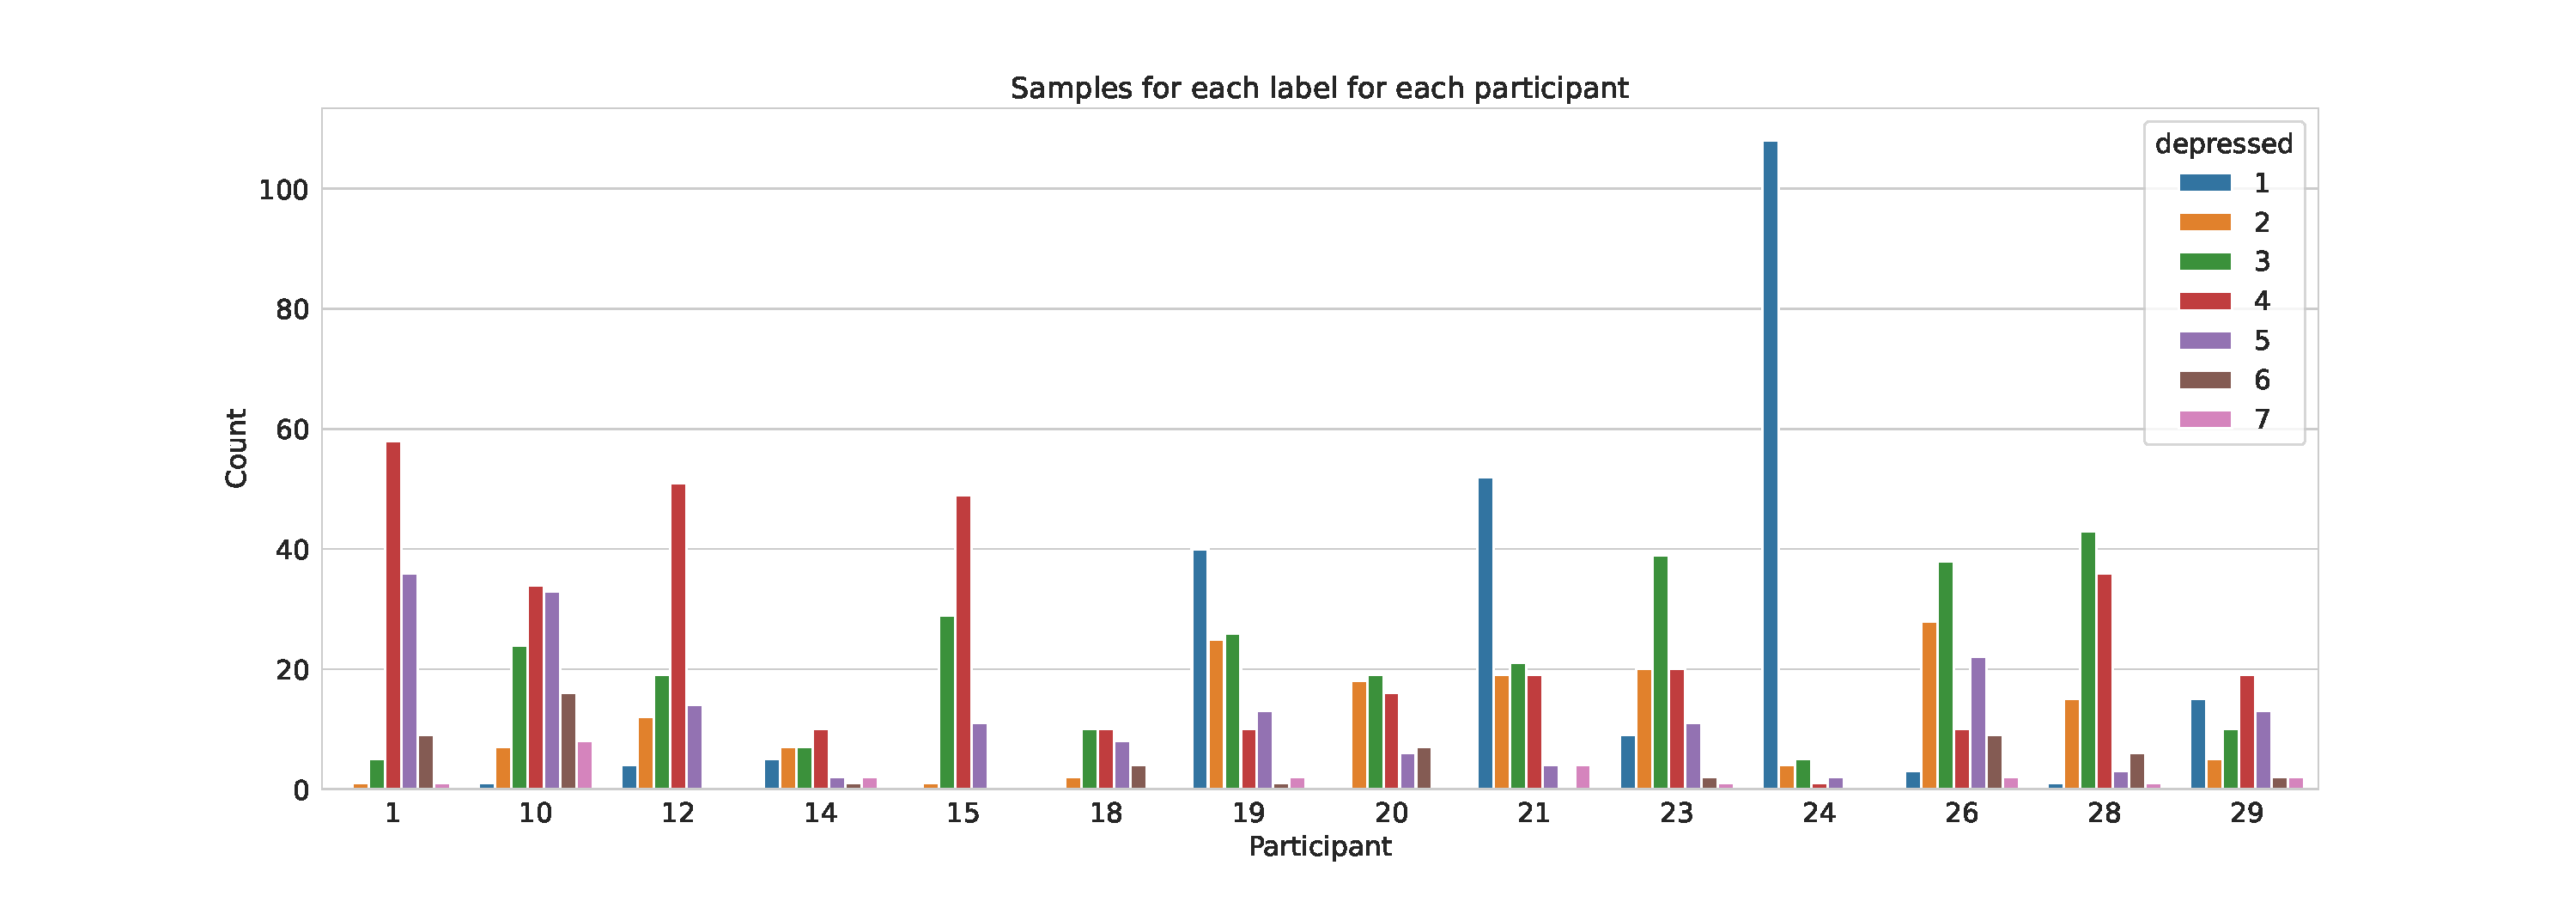
\includegraphics[width=\linewidth]{depression/fig/samples_by_labels.pdf}
    \caption{Number of label classes (depressed state values) per participant.}
    \label{fig:samples_by_labels}
\end{figure} 



As seen from Table \ref{tab:samples_participant}, 9 out of 14 participants have features where some values are missing. This could be due to device error or participant behaviour (e.g. a participant may forget to wear the smartwatch for a few hours). The \emph{Missing Values} column in the table represents the total number of missing data points, not the number of missing samples. For instance, there could be a sample where 4 of the feature data points are missing. The \emph{Features} column contains the number of features that have missing data points. A feature could be missing more than one data point across samples. Thus, the \emph{Missing Values} column shows the number of missing data points out of all the data points for the participant, which is 43 (number of features) times the total number of samples. However, there are no samples where all the feature values/data points are missing. Another information of interest is the total number of samples. Participants 14, 18, 21 and 29 have fewer samples and can be expected to perform poorly on deep learning models \cite{goodfellow_deep_2016}. 


\begin{table}[H] 
 \caption{Summary of Samples for each participant}
 \newcolumntype{C}{>{\centering\arraybackslash}p{0.2\textwidth}}
 \begin{tabular*}{\textwidth}{CCCCC}
 \toprule
 \textbf{Paricipant} & \textbf{Total Samples} & \textbf{Missing Values (Out of 43 x Total Samples)} & \textbf{Features w/ missing values} \\
 \midrule
 1 & 110 & 28 & 1\\
 10 & 123 & 108 & 27\\
 12 & 100 & 116 & 31 \\
 14 & 34 & 1 & 1\\
 15 & 90 & 0 & 0\\
 18 & 34 & 0 & 0\\
 19 & 117 & 18 & 1\\
 20 & 66 & 11 & 1\\
 21 & 119 & 0 & 0\\
 23 & 102 & 0 & 0 \\
 24 & 120 & 21 & 1\\
 26 & 112 & 10 & 4\\
 28 & 105 & 0 & 0\\
 29 & 66 & 9 & 1\\
 \bottomrule
 \end{tabular*}
 \label{tab:samples_participant}
\end{table}



Also, we noticed that some features for some participants are constant values, i.e., the same value repeats for each sample. This may make sense for neurocognitive assessment features (where a participant may perform consistently on the tests), but not for features acquired through the smartwatch. For instance, a participant would be highly unlikely to have the same non-zero value for \emph{exercise\ calorie} for 30 days. For instance, for some participants (participants 10, 15, 18, 21, and 23), the HRV feature titled \emph{ppg\_std} contained what appeared to be a missing or invalid value. The HRV feature indicates the standard deviation of PPG values captured from the Samsung Galaxy smartwatch's sensor within a ± 15-minute window around each depressed mood EMA. The value shown was consistently 999, which we deemed the default value recorded if an error or missing value scenario occurred. Similarly, for participants 18 and 24, 2 physical activity and sleep-based features titled \emph{exercise\_calorie}, \emph{exercise\_duration}, and \emph{prev\_night\_sleep} all recorded a value of 999 for every entry.




Moreover, we can see from Figure \ref{fig:samples_by_labels} that the label classes (depressed state values) across participants are not balanced. This is expected as the participants are mild-moderately depressed, and the higher ends of the depressed mood scale (which corresponds to severe depression) will be rarely represented. This imbalance, however, requires that special metrics be used when evaluating the model performance \cite{fernandez_performance_2018}. 



\subsection{Data Preprocessing}
\label{sec:data_preprocessing}
The previous section showed how the dataset contained not only missing data points but also columns with a single unique value. The dataset in its present state cannot be used for training, as most Machine Learning models do not accept datasets with missing values. Furthermore, training a model on a dataset where certain features have uncharacteristically unique values can confound the model and produce erroneous models. Hence, we preprocess the data. As different data preprocessing methods have advantages and disadvantages, we try three data preprocessing methods and build models for each to compare which method suits the dataset.

For the first method, we use \emph{Deletion} as follows:
\begin{itemize}
 \item Identify participants for whom we have constant feature values for features acquired from the smartwatch - call it set \emph{C}.
 \item Remove participants in \emph{C}.
 \item Identify (from remaining participants) those participants for whom we have missing data points - call it set \emph{M}.
 \item For participants in \emph{M}, remove the samples containing the missing data points.
\end{itemize}

The aim in this method is to ensure that each participant has all 43 features with no missing data points. For the first portion of the goal, we remove the participants with constant smartwatch feature values. This step eliminates participants 10, 15, 18, 21, 23 and 24. For the second portion of the goal, we remove the samples/rows with any missing data. This step will reduce the number of samples for some participants. However, this deletion method is the most straightforward data preprocessing method and provides a good baseline against sophisticated data preprocessing methods.


For the second method, we use a \emph{Manual Imputation} technique using a set of differentiated data preprocessing steps as follows:
\begin{itemize}
 \item Identify participants for whom we have constant feature values for features acquired from the smartwatch - call it set \emph{C}.
 \item Remove the features with constant values for participants in \emph{C}
 \item Identify participants for whom we have missing data points - call it set \emph{M}.
 \item For participants in \emph{M}, identify the features with missing data points - call it set \emph{F}.
 \item Identify if the features in set \emph{F} contain discrete, continuous or neurocognitive values. 
 \item For discrete features, the missing values are filled with the most frequent value.
 \item For continuous features, the missing values are imputed using an Iterative Imputer (see Table \ref{tab:missing_data_methods}).
 \item For neurocognitive features, we fill in the missing values with zero.
\end{itemize}

This method chooses the methods used to impute/fill data by the data type. It imputes the missing values with the most frequent value for discrete values. In contrast, for continuous values, it imputes the missing values using an iterative method that computes the missing values in each feature by considering it as a function of all other features in a round-robin manner. We use the iterative imputer for continuous variables as it tries to preserve the influence of other features on the feature with missing values \cite{buck_method_1960}. Finally, we impute the missing values in the neurocognitive features with zero. The neurocognitive features are assessment-based, and imputing missing values with zero seems acceptable, as a zero in an assessment typically implies an empty/void assessment. This method is similar to what is presented in \cite{shah_personalized_2021}.


For the third method, we employ \emph{Automatic Imputation} using a set of sophisticated data preprocessing steps as follows:
\begin{itemize}
 \item Identify participants for whom we have constant feature values for features acquired from the smartwatch - call it set \emph{C}.
 \item Remove the features with constant values for participants in \emph{C}
 \item Identify participants for whom we have missing data points - call it set \emph{M}.
 \item For participants in \emph{M}, identify the features with missing data points - call it set \emph{F}.
 \item For each feature in \emph{F}, fill in the missing values with different data-filling methods, one at a time.
 \item Choose the data-filling method that gives a data distribution that best matches the data distribution before any preprocessing.
\end{itemize}

This method aims to remove any confounding features while preserving as many samples as possible by filling in missing data. For the first part, we remove the features with constant feature values. Next, we handle missing data by choosing a data-filling method that changes the data distribution the least. Instead of manually choosing an appropriate method, we automate the process and use seven different data-filling methods for each feature with missing values. The chosen methods are summarised in Table \ref{tab:missing_data_methods}. 


\begin{table}[h] 
 \caption{Summary of methods used for handling missing data in a feature column}
\newcolumntype{P}{>{\raggedright\arraybackslash}p{0.25\textwidth}}
\newcolumntype{L}{>{\raggedright\arraybackslash}p{0.75\textwidth}}
 \begin{tabular*}{\textwidth}{PL}
 \toprule
 \textbf{Method} & \textbf{Description}\\
 \midrule
 Mean & Fill missing data with the mean of the available data \\
 Median & Fill missing data with the median of the available data\\
 Forward Fill & Fill missing data by continuing the last available data\\
 Backward Fill & Fill missing data by continuing the next available data\\
 Linear Interpolation & Fill missing data through linear interpolation using the data points before and after the missing data\\
 Iterative Imputation \cite{buuren_mice_2011} & A strategy for imputing missing values by modelling each feature with missing values as a function of other features in a round-robin fashion. This method only uses samples with no missing data as input (in case multiple features in a dataset have missing values) \\
 KNN Imputation \cite{troyanskaya_missing_2001} & Each sample's missing values are imputed using the mean value from some nearest neighbours found in the training set. Two samples are close if the features that are not missing in either are close.\\
 \bottomrule
 \end{tabular*}
 \label{tab:missing_data_methods}
\end{table}


Finally, we compare the methods using the distribution of the filled-in feature and the original feature vectors. For this, we use the Two-sample Kolmogorov-Smirnov (KS) test, which compares two distributions by finding the maximum difference between the Cumulative Distribution Functions (CDFs) of the two distributions \cite{hodges_significance_1958}. In general, the KS test is used to compare the underlying continuous distributions F(x) and G(x) of two independent samples. This statistical test uses the null hypothesis that the two distributions are identical, i.e. F(x)=G(x) for all x. The alternative hypothesis is that they are not identical. The test produces a \emph{statistic} and a \emph{p-value} \cite{bruce_statistical_2017}. The \emph{statistic} obtained from the test is the maximum absolute difference between the empirical distribution functions of the samples. 

We choose a confidence level of 95\%; i.e. we reject the null hypothesis in favour of the alternative if the \emph{p-value} is less than 0.05. The higher the \emph{p-value}, the more probable the fact that the two distributions (i.e., before and after data filling) are similar and not just due to chance. Thus, we choose a method with the highest \emph{p-value} and low \emph{statistic}. As different methods are chosen for different features for every participant, we decided against reporting them here to maintain the succinctness of the chapter.



   
   
   

\section{Monolithic Model Development}
\label{sec:monolithic_model_development}
Since the depression scale is ordinal, i.e. there is an order in the value of the depression/mood score, and it ranges between 1 and 7, we can consider the mood score prediction problem as either a regression or classification problem. As a regression problem, the model will be concerned with developing a model that predicts values that are close to the actual mood scores. A classification model, on the other hand, considers the mood scores as seven classes and tries to predict a class based on the input. 

First, we use ten common regression and classification classical ML models to build baseline models against which to compare the performance of MLP models. Then, we use MLP models to build the regression and classification models. Moreover, we build models for the MLP regression and classification models for the different types of data imputation schemes (see Section \ref{sec:data_preprocessing}). The whole model development framework\footnote{Although we experiment with only MLP models in this work, the methodology is model agnostic and can be applied to other ML models too by replacing the MLP model with another ML model.}  is shown in Figure \ref{fig:monolithic_model_framework}.



\begin{figure}[htbp] 
  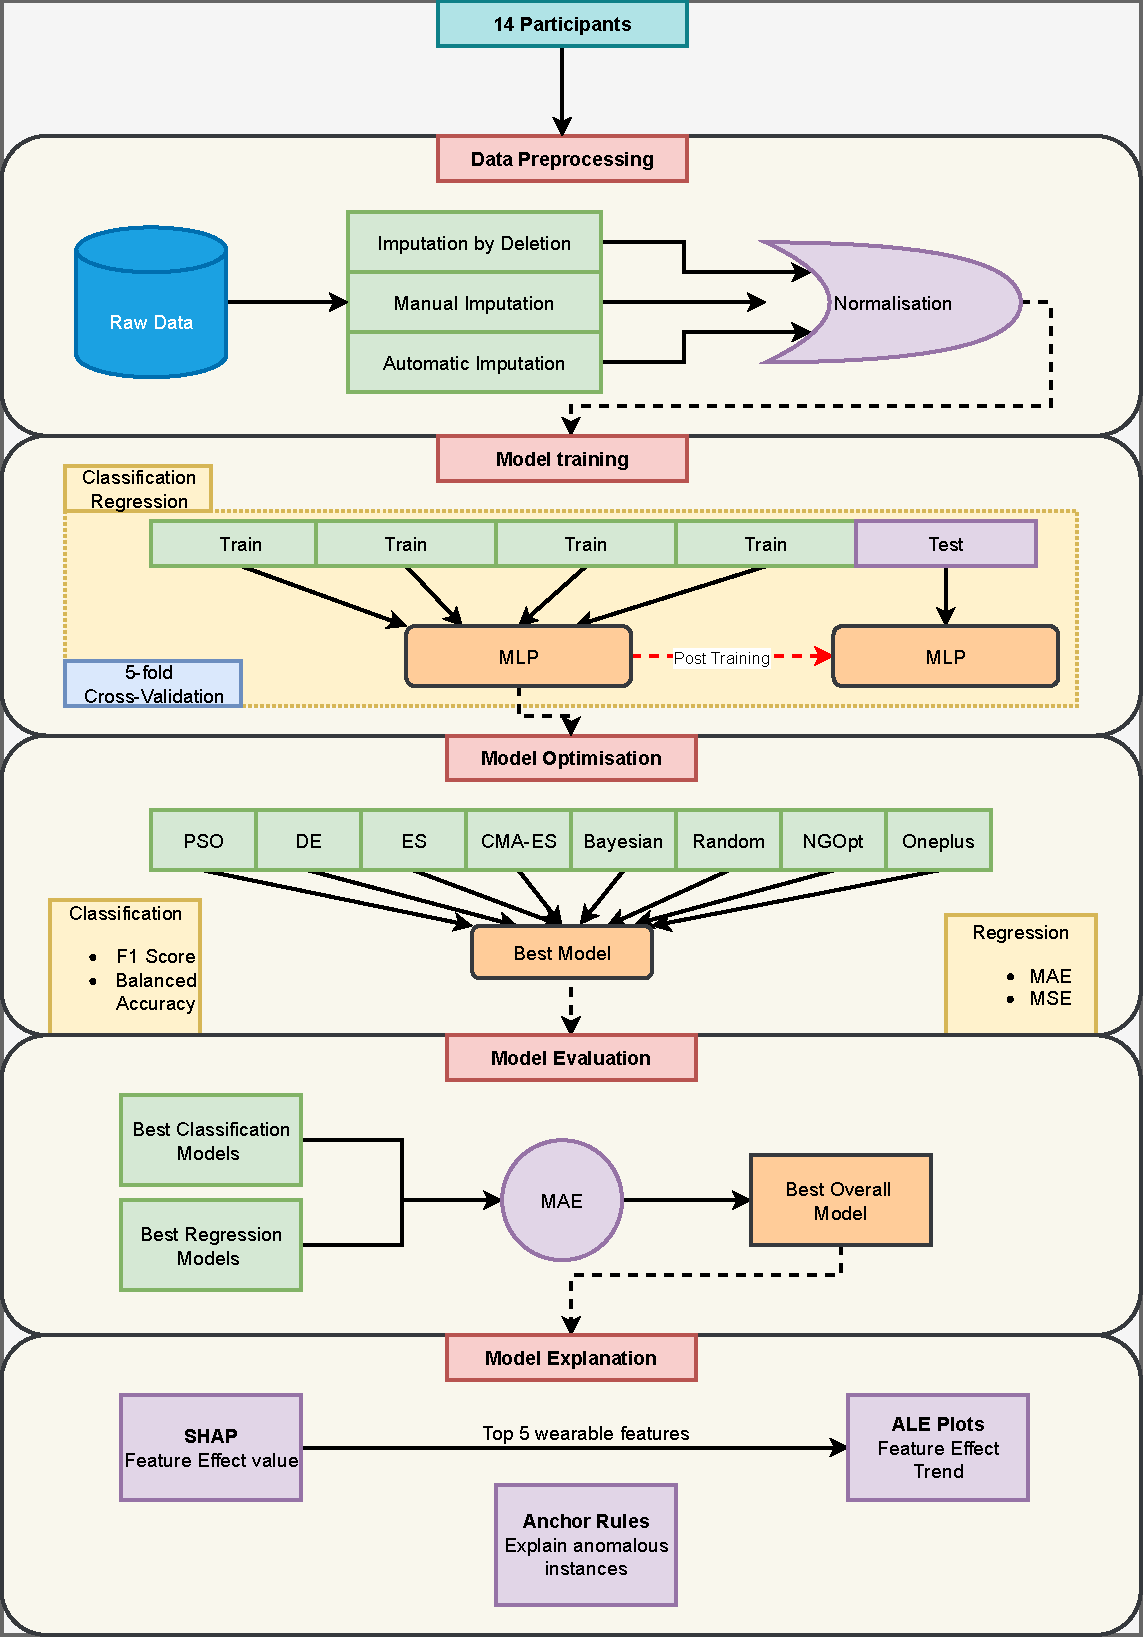
\includegraphics[width=15.5cm]{depression/fig/ModelFramework.pdf}
  \caption{The Personalised Mood Score Prediction Framework for monolithic models. This framework is repeated for all 14 participants. We begin at the top with data preprocessing. The preprocessed data is then used for model training of classification- and regression-based MLP models. The Best models from the classification and regression training and optimisation are compared to find the best overall models with minimum \gls{mae} (MAE). This best overall model is then used to get model explanations using SHAP, ALE plots and Anchor rules.}
  \label{fig:monolithic_model_framework}
\end{figure}  
  


\subsection{Base Models}
\label{sec:base_model}
We built a set of base models to act as a baseline for the predictive performance of MLP models on the dataset. We trained ten common classical ML algorithms  (eight of which were used in~\cite{shah_personalized_2021}) on the three preprocessed datasets for each participant: Adaboost Regressor, Adaboost Classifier, Elasticnet Regressor, Gradient Boosting Classifier, Gradient Boosting Regressor, Poisson Regressor, Random Forest Classifier, Random Forest Regressor, Support Vector Classifier and Support Vector Regressor. Also, we used a simple grid search (as used in~\cite{shah_personalized_2021}) to tune the hyperparameters of the models. The grid search is a brute-force method that tries all possible combinations of hyperparameters and chooses the combination that provides the best prediction performance. 

Furthermore, a Stratified 5-fold Cross-Validation (CV) scheme was used to validate the model performance during and after training. This scheme divides the normalised dataset into five parts, trains a model on the four parts (the training dataset) and tests on the remaining part (the testing dataset). It does so in a round-robin fashion. The division is stratified, meaning each fold contains the same proportion of the different output labels. So, for a 5-fold CV, we built five separate models (with the same architecture) on the five training and test datasets. The overall performance was obtained by taking the mean of the training and test performance values over the five sets. Also, the test datasets do not overlap between the folds. This method ensures that the evaluation of the model is free of data-selection bias, which may arise when using a simple train--test split, as the performance depends on the particular split of the train and test set. 

For each participant, the model (out of the ten) with the lowest Mean Absolute Error (MAE) after hyperparameter tuning, irrespective of classification or regression, was chosen as the base model. More details on the grid search and the hyperparameters used for each model are provided in Appendix \ref{sec:base_hyperparameters}. Note that the base models were only used for performance comparison with the MLP models and were not used for a model-explanation comparison, as the explainability of such models in a mood-prediction setting has been explored in~\cite{shah_personalized_2021}.


\subsection{MLP Model Architecture}
\label{sec:monolithic_model_architecture}
The model architecture differs between the regression and the classification models. As mentioned in the previous section, we use \glspl{dnn} (\glspl{mlp}) to build the model. While both models have an input layer, a few hidden layers, and an output layer, the number of neurons in the output layer differs between a regression model and a classification model. As a regression model predicts a single value for each input, all regression models use only one neuron in the output layer with \emph{no} activation. On the other hand, the classification models have seven neurons corresponding to the seven classes (mood scores). Outputs from the neurons are normalised (squashed) using a \emph{softmax} activation. These squashed values (for each neuron) lie between 0 and 1 and represent the probability of an input belonging to that class. The class corresponding to the highest output value is taken as the output. The MLP models (both classification and regression) comprise several MLP layers with some neurons in each layer. The actual number of layers, the number of neurons in each layer and the activation for each layer are determined by an optimisation algorithm described in Section \ref{sec:model_optimisation}.




\subsection{Model Training}
\label{sec:monolithic_model_training}
All models are built and trained in Python using the TensorFlow-Keras library, which uses a loss function and an optimiser. The loss function is a function that evaluates the model prediction against the actual output value and produces a numeric value based on how different or similar the prediction and the actual values are. Moreover, the optimiser optimises/modifies the weights/parameters of the DNNs so that the loss is minimised. For the classification models, we use a version of the cross-entropy loss (see Equation \ref{eq:crossentropy}) called the \emph{Sparse Categorical Crossentropy}. The regression models use either the \gls{mse} or the \gls{mae} between the predicted and actual values as the loss function. We use a version of stochastic gradient descent called \emph{Adam} optimiser to optimise the loss function of all models. 



Also, the preprocessed dataset is time-sorted and normalised before it is fed into the models for training. This ensures smoother convergence of the loss function. We use the standard normalisation procedure. It centres the data around zero and gives the dataset's unit standard deviation. This is achieved by subtracting the feature means from each feature and dividing the result by the standard deviation of the feature (see Equation \ref{eq:standard_scaler}).


We use a Stratified 5-fold \gls{cv} scheme to validate the model performance during and after training. The samples in the normalised folds are then randomised and fed into the MLP models for training, i.e. the MLP models take an input of shape $N \times F$, where $N$ is the number of input samples (data points) and $F$ is the number of features. Moreover, we follow these steps for all MLP models built for both regression and classification, irrespective of the data imputation method. We train each model using batches of training data for 100 epochs, i.e. for 100 iterations of the entire training data (divided into batches). We also only save the best model across the epochs and use the early-stopping strategy, which stops the training before the epochs finish if the model's performance does not improve for a certain number of epochs. 




\subsection{Model Optimisation}
\label{sec:model_optimisation}
It is usually challenging to infer the architecture of the DNN that gives the best possible performance, and there are often multiple parameters that influence the performance of a DNN. Hence, we decided to further optimise the model hyperparameters (i.e. the extrinsic model parameters that influence performance, such as the model architecture and training) using multiple Evolutionary Algorithm (EA) based schemes and stochastic schemes to obtain better model performance. 



\begin{table}[htbp] 
 \caption{Summary of optimisation algorithms/methods used in hyperparameter optimisation}
 \newcolumntype{P}{>{\raggedright\arraybackslash}p{0.2\linewidth}}
 \newcolumntype{F}{>{\raggedright\arraybackslash}p{0.55\linewidth}}
 \newcolumntype{L}{>{\raggedright\arraybackslash}p{0.2\linewidth}}
 \begin{tabular*}{\textwidth}{PFL}
 \toprule
 \textbf{Algorithm} & \textbf{Summary} & \textbf{Parameters} \\
 \midrule
 \gls{pso} \cite{zambrano-bigiarini_standard_2013} & Particle Swarm Optimisation of the loss on hyperparameters based on a set of particles (candidate solutions) with their inertia & Population Size: 10 \\
 \gls{de} \cite{price_differential_2005} & Differential Evolution-based optimisation. It uses differences between points in the population (candidate solution) for doing mutations in fruitful directions & Population Size: 10 \\
 \gls{es} \cite{emmerich_evolution_2018} & Evolution Strategy-based optimisation of hyperparameters is based on the ideas of evolution & Population Size: 10\\
 \gls{cmaes} \cite{emmerich_evolution_2018} & Covariance Matrix Adaptation Evolutionary Strategy is a variation of ES where the covariance matrix of the distribution is incrementally updated to increase the likelihood of previously successful search steps & Population Size: 10\\
 Random & Random search of the hyperparameter space & N.A \\
 Bayesian \cite{raponi_high_2020} & Bayesian Optimisation of the loss on hyperparameters. Optimisation on search space depends on the initialisation type & Initialisation: Latin Hypercube Sampling \\
 \gls{ngopt} \cite{rapin_nevergrad_2018} & Nevergrad Library's own optimiser & N.A \\
 Oneplusone \cite{rapin_nevergrad_2018} & 1+1 optimisation of the loss on the hyperparameter space & N.A\\
 \bottomrule
 \end{tabular*}
 \label{tab:optimiser_types}
\end{table}


We use eight different EAs and statistical methods to optimise the number of hidden layers in the model, the maximum number of neurons, the activation of the hidden layers, and the batch size of the training. We optimise the maximum number of neurons and not the number of neurons in each layer, as that would have increased the number of optimisation variables. Increasing the number of optimisation variables increases the optimisation space, making the optimisation problem more difficult. We linearly interpolate the neurons in the hidden layers (whose number is also optimised) using the maximum number of neurons and the number of neurons in the output layer (which depends on whether the model is classification or regression). The eight EA methods we use, and their parameters, are mentioned in Table \ref{tab:optimiser_types}. Table \ref{tab:optimiser_values} also contains upper and lower limits for each hyperparameter used during the optimisation.



\begin{table}[htbp] 
 \caption{Search values (or limits) for parameters during hyperparameter optimisation}
 \begin{tabular}{p{0.3\linewidth}p{0.2\linewidth}p{0.2\linewidth}p{0.2\linewidth}}
 \toprule
 \textbf{Hyperparameter} & \textbf{Lower Limit} & \textbf{Upper Limit} & \textbf{Values}\\
 \midrule
 Number of layers & 2 & 4 & N.A\\
 Maximum number of neurons & 30 & 60 & N.A \\
 Activation & N.A & N.A & \gls{tanh}, \gls{relu}, \gls{elu}, linear\\
 Batch size & N.A & N.A & 4, 6, 8 \\
 \bottomrule
 \end{tabular}
 \label{tab:monolithic_optimiser_values}
\end{table}



Figure \ref{fig:model_optimisation} shows the optimisation schematic. Hyperparameter optimisation exists as an outer loop in the inner loop of model training (which optimises the model weights). The optimisation repeats over several iterations, during which the model is trained using the 5-fold CV procedure. We average the model performance over the five folds and use that as the performance metric to optimise the hyperparameters. We use the metrics F1-score and \emph{\gls{ba}} to optimise the classification models and use \gls{mse} and \gls{mae} to optimise the regression models. We optimise the classification models to reduce the margin between the perfect performance (100\% accuracy, for instance) and the performance obtained from the model. For the regression models, we minimise the metrics as they are error-based.


\begin{figure}[htbp] 
 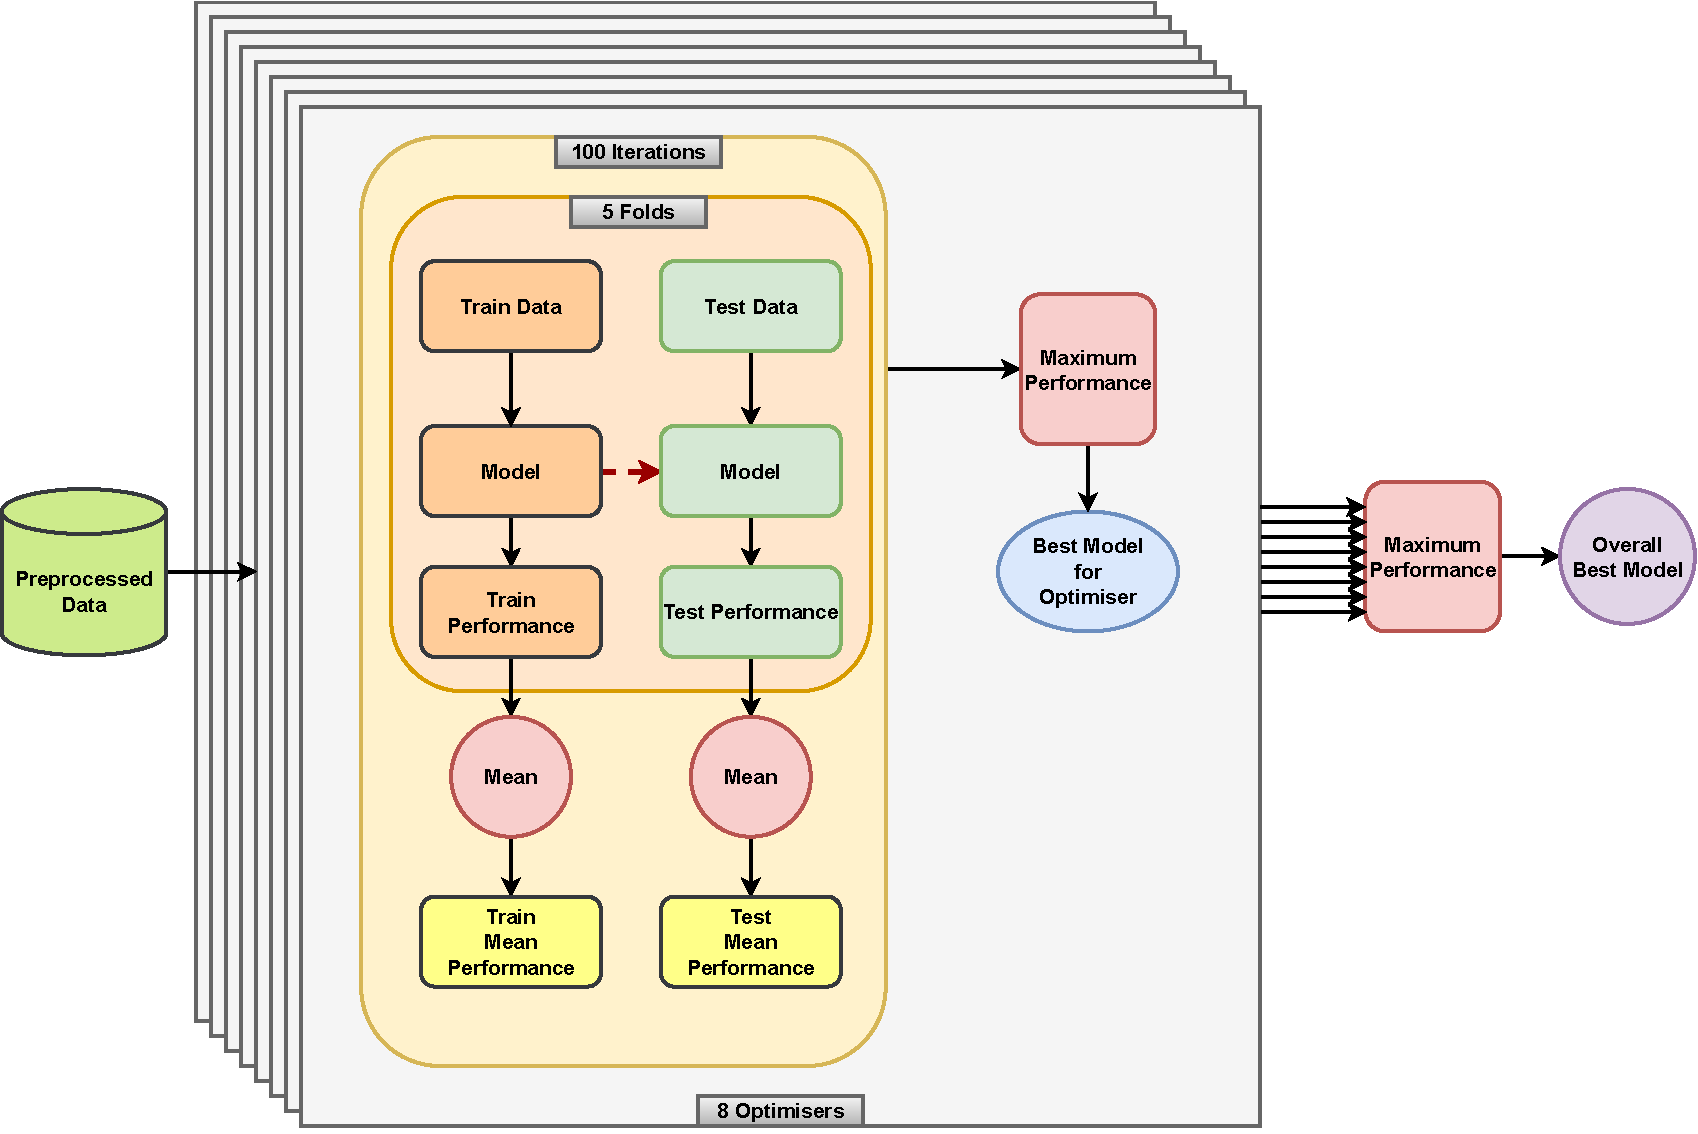
\includegraphics[width=\linewidth]{depression/fig/ShahOptimisation.pdf}
 \caption{The Optimisation Procedure.}
 \label{fig:model_optimisation}
\end{figure}


We run the optimisation for 100 iterations for all methods. At the end of the 100 iterations, we take the best models, i.e. models with the best mean 5-fold performance, from each method and find the best among the eight best (one for each optimisation method) models as well. We use the same metrics to optimise the hyperparameters to find the best models. The performance of these best models is then taken as the best for a particular combination of optimisation metric, problem type and data imputation method. 

The optimisation procedure is entirely parallelised, and the number of parallel processes is determined by the number of cores in the system used for optimisation and training. We run the optimisation (and training) in a Docker Ubuntu container containing all the required Python libraries, such as TensorFlow-Keras (for training the models) \cite{martin_abadi_tensorflow_2015} and Nevergrad (for the optimisation) \cite{rapin_nevergrad_2018}. Parallelisation reduces the optimisation time significantly, making the procedure scalable to a high number of optimisation iterations. 


\subsection{Model Evaluation and Explanation}
\label{sec:monolithic_model_evaluation}
We gather the best model for each combination of problem type (classification or regression), data preprocessing methodology and metric used for hyperparameter optimisation (i.e. 12 combinations). As both regression and classification problems use different performance metrics except for \gls{mae}, to find the best overall method, we use \gls{mae} as it corresponds to the absolute error. Hence, for each participant, we collect the best models from the 12 combinations, find the model with the lowest test \gls{mae}, and use it as the overall best-optimised model.

This overall best model is the final model for the participant, and we use this to extract important indicators/features and explain how those indicators affect mood. To this end, we use three post-hoc explainability methods from the \gls{xai} literature \cite{molnar_interpretable_nodate}. We use \gls{shap} \cite{lundberg_unified_2017}, \gls{ale} plots \cite{apley_visualizing_2019} and Anchors \cite{ribeiro_anchors_2018}. All explanation methods take the unnormalised data as input (which is internally normalised before being fed into the models). Using unnormalised data ensures that the explanations are produced in the actual data range, which makes it easier to interpret.

Here, we used \gls{shap} to find the top five important features of each participant. We got one \gls{shap} value per data instance per feature, and to compute global feature importance for a model and a dataset, we took the mean of the absolute \gls{shap} values for all instances in the dataset to obtain the overall \gls{shap} value of a feature. Also, as we used a 5-fold \gls{cv} approach, we found the \gls{shap} values for each fold and averaged them. As with \gls{shap}, we used the test dataset to compute the \gls{ale} value for each fold and found the overall \gls{ale} value by taking the mean of the \gls{ale} values obtained for the five folds. Finally, we used Anchors to show how specific predictions for models could be explained in a rule-based manner.


\section{Compositional Model Development}
\label{sec:compositional_model_development}


\subsection{Compositional Modelling Overview}

In the following sections, we present the design of compositional models. As the name suggests, a compositional model comprises multiple sub-models whose outputs are combined to produce a single output. It is a modular modelling paradigm that promotes using multiple smaller models that should be easier to explain, especially for complex ML models. 

Typically, sub-models in a compositional model are built on data obtained by segregating the complete dataset with its complete input feature/predictor set into subsets of features. We call this subset a cluster. Each sub-model reasons on its cluster. The outputs from the sub-models can be combined/composed hierarchically using \emph{Merge} models to form the complete compositional model. This hierarchical multi-staged design gives more control over the flow of data and makes it more transparent. The compositional model and the sub-models can be trained to reason on the same set of outputs or different outputs based on design requirements. 

In the personalised mood score prediction case, the compositional model consists of sub-models that are built on clusters obtained from the dataset described in Section \ref{sec:depression_data}. The goal of both the compositional model and the sub-models is to predict the mood state of a depressed participant, given a set of input features. Each compositional model learns to predict the mood state given a subset of features (cluster) from the complete dataset. It, therefore, learns the relationships between the features contained in its cluster. We combine the outputs of all sub-models, which have learned representations for their cluster, in a specific hierarchical architecture to form the compositional model. Thus, the compositional designs learn separate representations and the relationships between those representations, and so on, based on the compositional architecture.

For example, consider Equation {\ref{eq:comp_model_example}}, where the compositional model architecture consists of four initial models ($Models_1, \dots, Models_4$) that receive inputs from their feature clusters ($cluster_1, \dots, cluster_4$). These models are combined hierarchically using three Merge models -- $M_{1}^{stage1}$, $M_{2}^{stage1}$, and $M^{stage2}_1$ in two stages. First, $M_{1}^{stage1}$ and $M_{2}^{stage1}$ combine the outputs of the four initial models. The model outputs from the two Merge models are then combined to produce the final output $M^{stage2}_1$. 

\begin{multline}
    \begin{aligned}
 Output = M^{stage2}_1(M^{stage1}_1(Model_1(cluster_1) + Model_2(cluster_2)) + \\
 (M^{stage1}_2(Model_3(cluster_3) + Model_4(cluster_4)))
    \label{eq:comp_model_example}
    \end{aligned}
\end{multline}

Additionally, similar to the monolithic model, the mood scores may be formulated either as a regression task or as a classification task \cite{murphy_machine_2012}, and all models are evaluated under multiple data-imputation strategies (see Section \ref{sec:data_preprocessing}). The overall MLP development pipeline\footnote{Although we experiment with only MLP models in this work, the methodology is model agnostic and can be applied to other ML models too by replacing the MLP model with another ML model.} is illustrated in Figure \ref{fig:model_framework}.  


\begin{figure}[htbp]
  \centering
  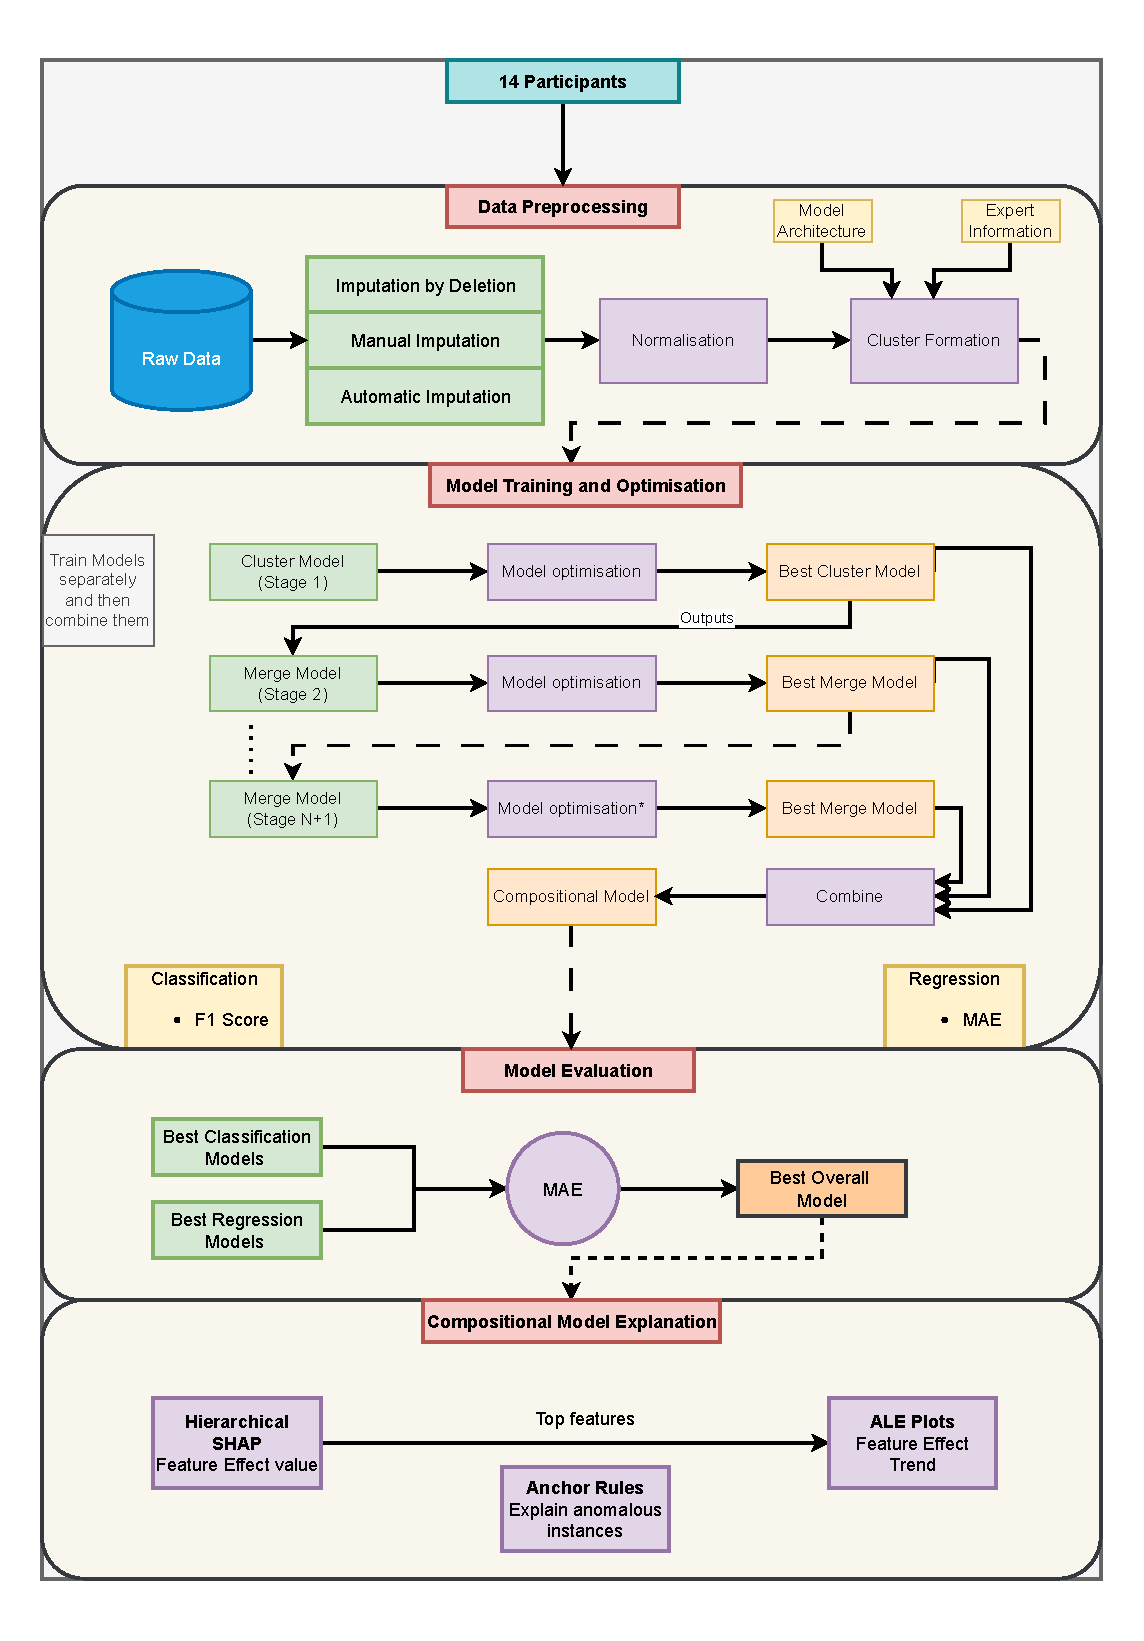
\includegraphics[scale=0.8]{depression/fig/ModelFramework_2.pdf}
  \caption{The proposed Personalised Mood Score Prediction Framework for the compositional models. This framework is repeated for all 14 participants. We begin at the top with data preprocessing. The preprocessed data is then used to train classification- and regression-based MLP compositional models. The Best compositional models from the classification and regression training (using 5-fold Cross-Validation) and optimisation are compared to find the best overall models with minimum \gls{mae} (MAE). This best overall model is then used to get model explanations using SHAP, ALE plots and Anchor rules.}
  \label{fig:model_framework}
\end{figure}


\subsection{Compositional Model Architecture}
\label{sec:compositional_model_architecture}

The compositional model (regardless of regression or classification) will always be a funnel-like design with multiple stages, and the number of models per stage decreases as we approach the output. We call the models in the first stage Cluster models, and the models in subsequent stages Merge models. At each stage (except for Stage 1, where the biophysical signals are used as inputs), the outputs from models in the previous stage are used as inputs. 

The number of clusters, the features in those clusters, and the subsequent number of combination models and stages are all parameters that have to be based on either expert knowledge or experimentation. In this work, we consider multiple possible approaches to form the clusters and the model architecture to explore which approach offers a design with the best performance and explanation. We choose these approaches based on differences in data sources and expert opinion. 

Specifically, we consider three different architectures: (1) a design with six cluster models, one Merge model and two stages; (2) a design with three cluster models, two Merge models and three stages; and (3) a design with ten cluster models, three Merge models and three stages. We cannot consider all combinations and only consider a few decompositions to explore the possible advantages and disadvantages of the compositional model.




\subsubsection{Approach 1: Compositional Model with 2 Stages and six cluster models}

\begin{figure}[htbp]
\centering
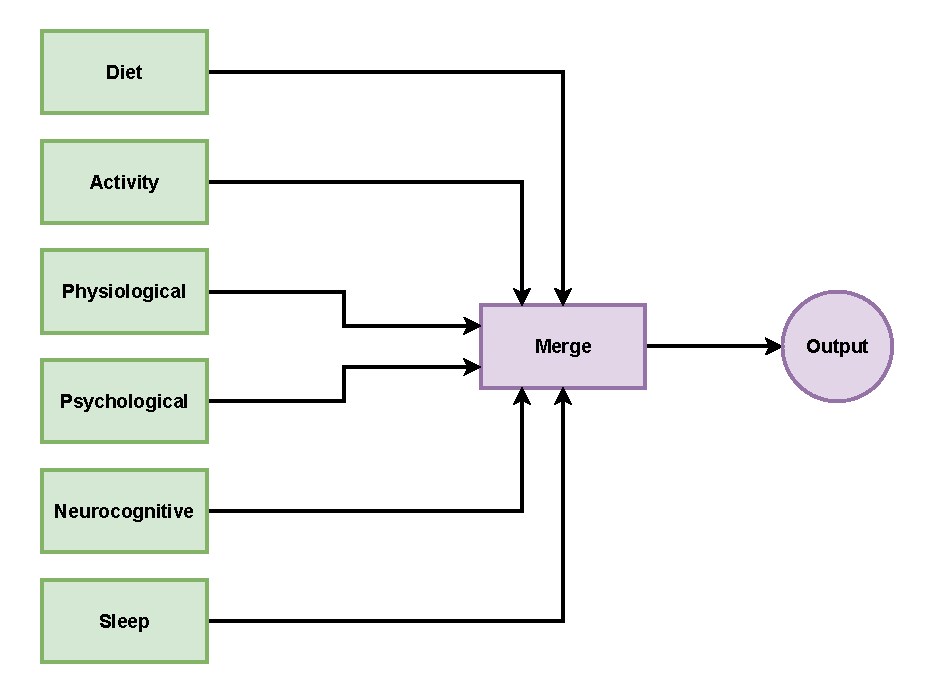
\includegraphics[width = \linewidth]{depression/fig/Shah_model_2Stages.pdf}
\caption{Compositional model with six clusters and two stages.}
\label{fig:comp_6}
\end{figure}

The first architecture we consider consists of six MLP cluster models. The design is shown in Figure \ref{fig:comp_6}. Here, we divide the clusters based on the source of data - Activity, Diet, Physiological, Psychological, Sleep and Neurocognitive. The Activity cluster contains data from wearables that record the activity (exercise) of the participants. The Diet cluster contains data from smartwatches where individuals record their food consumption (particularly sugar, caffeine, and fat consumption). 

\begin{equation}
    \hat{y} = \sum_{i=1}^{6} w_i \hat{y}_i
\label{eq:comp_3}
\end{equation}


Moreover, the physiological cluster contains data from wearables that record cardiovascular data, e.g. heart rate, breathing rate, etc. The psychological cluster contains data from the smartwatch where individuals record features that reflect the psychological factors affecting mood, such as anxiety and distraction. The sleep cluster contains data from wearables that record the sleep patterns of the participants. Currently, we only have one sleep feature - the previous night's sleep. The Neurocognitive cluster contains data from Neurocognitive tests conducted in the clinic. The Merge model combines the outputs from the cluster models using a white-box weighted average function (see Equation \ref{eq:comp_3}), whose weights the model learns. All feature names corresponding to the cluster models are given in Appendix \ref{sec:appendix_model_features}.


\subsubsection{Approach 2: Compositional Model with 3 Stages and three cluster models}

\begin{figure}[htbp]
\centering
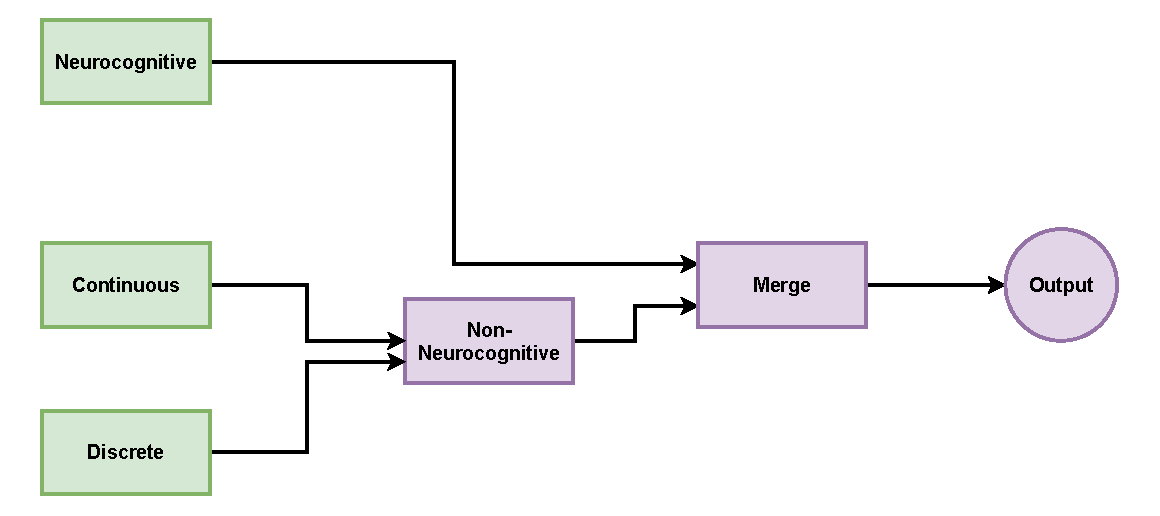
\includegraphics[width = \linewidth]{depression/fig/Shah_model_3stages.pdf}
\caption{Compositional model with three clusters and two stages.}
\label{fig:comp_7}
\end{figure}

The second architecture we consider consists of three MLP cluster models and three stages. The design is shown in Figure \ref{fig:comp_7}. Here, we divide the clusters based on the kind of data: Continuous, Discrete, and Neurocognitive. The Continuous cluster contains continuous data from wearables that record the activity (exercise), heart rate, and sleep data of the participants. The Discrete cluster contains data from the EMA recordings, such as the anxiety level, number of cups of coffee, etc. The Neurocognitive cluster contains data from Neurocognitive tests conducted in the clinic. 

Here, we have two Merge models. The first Merge model, called Non-Neurocognitive, combines the outputs of the Continuous and Discrete cluster models. The second Merge model combines the outputs from the Non-Neurocognitive Merge models and the Neurocognitive cluster model. Both Merge models are MLP models. The output of the final merge block is the final prediction of the model. All feature names corresponding to the cluster models are given in Appendix \ref{sec:appendix_model_features}.



\subsubsection{Approach 3: Compositional Model with 3 Stages and 10 cluster models}

The third architecture we consider is a three-stage architecture with three cluster models. It is shown in Figure \ref{fig:comp_3_stage}. Here, we begin by dividing the features into three super-clusters based on the source of data: Smartwatch, EMA, and Neurocognitive. Then, we subdivide the super-clusters into smaller clusters. The Smartwatch super-cluster contains the Activity, Sleep, and Heart-based cluster models. The EMA super-cluster contains the Diet, Ema, and Breathing cluster models. The Neurocognitive super-cluster contains the Neurocognitive cluster models. 

\begin{figure}[htbp]
    \centering
    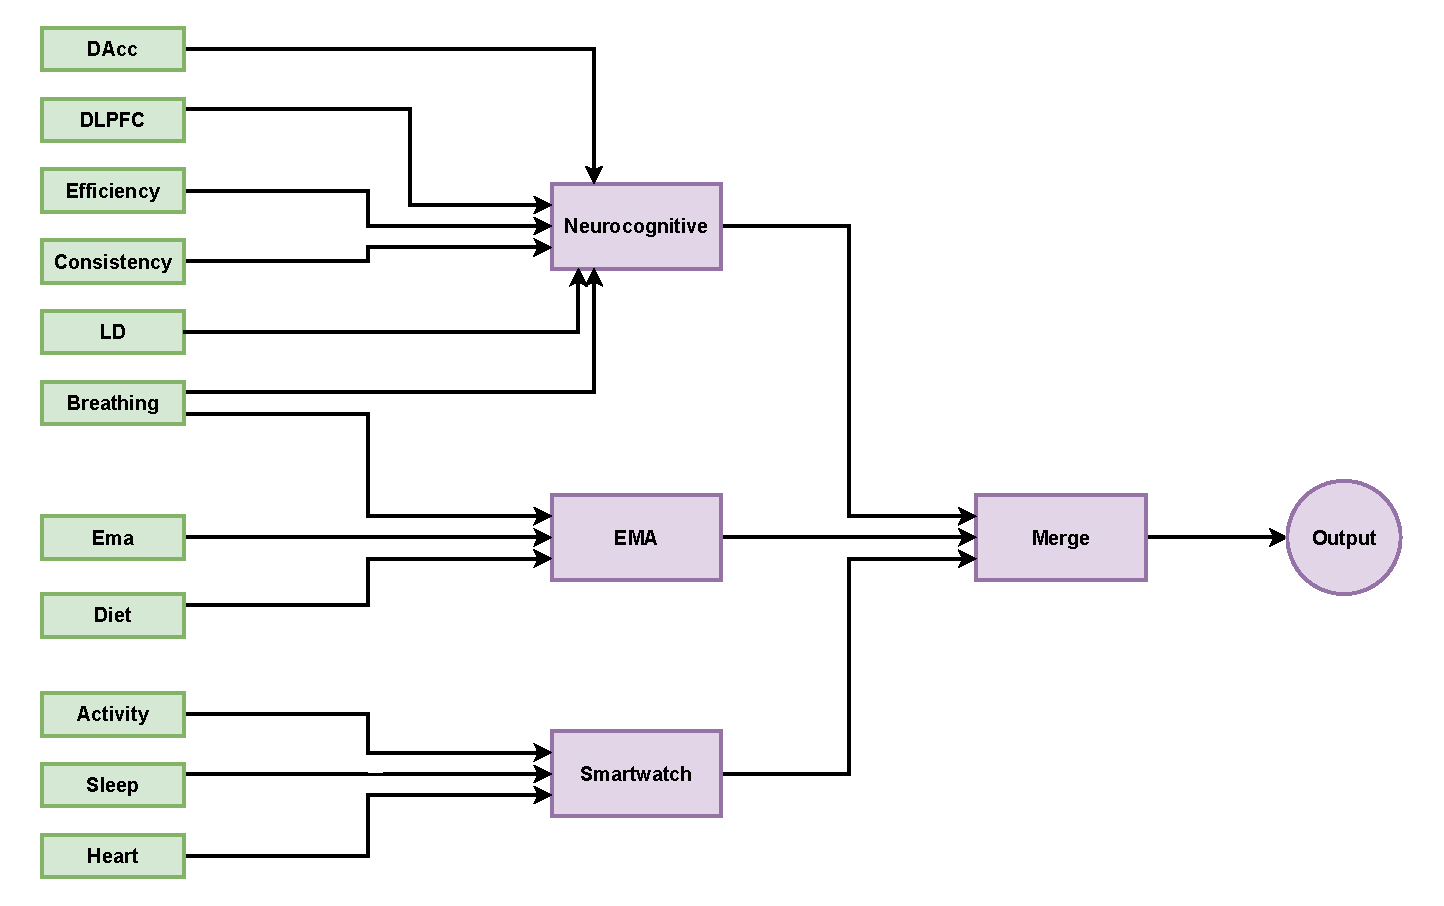
\includegraphics[width = \linewidth]{depression/fig/Shah_model_3stages_fred.pdf}
\caption{Compositional model with three stages and 3 cluster models.}
\label{fig:comp_3_stage}
\end{figure}

Overall, the first stage contains 10 MLP cluster models. These models in each super-cluster are combined into super-cluster-level MLP Merge models called Smartwatch, EMA, and Neurocognitive. This produces three Merge models in the second stage. These three Merge models are later combined into a final Merge model in the third stage. The output of the final merge block is the final prediction of the model.

To elaborate, the models feeding into the Neurocognitive Merge model correspond to the neurocognitive assessments performed on participants. \gls{dlpfc}, \gls{dacc} models correspond to features from recorded neural activity in these brain regions. \gls{ld} contains the reward metrics for the Lucky-Door game assessment. Breathing, Consistency and Efficiency contain features that measure the breathing, consistency and efficiency of participants in the assessments. All feature names corresponding to the cluster models are given in Appendix \ref{sec:appendix_model_features}.



\subsubsection{Regression and Classification Modelling}

Regression and Classification compositional models were constructed using the architectures mentioned thus far. In a classification (or regression) compositional model, every sub-model is also a classification (or regression) model. The regression models featured a single output neuron—without any activation function—to generate a continuous prediction for each input. In contrast, the classification models utilised seven output neurons, one per mood‐score category, each followed by a \textit{softmax} activation. The resulting normalised outputs, constrained to the interval \([0,1]\), represent class‐membership probabilities, and the class associated with the maximal probability is selected as the model's prediction. The precise network depth, the neuron counts per layer, and the choice of activation functions were all established via the hyperparameter optimisation procedure detailed in Section \ref{sec:compositional_model_training}.  



\subsection{Compositional Model Training}
\label{sec:compositional_model_training}

In a compositional model, each sub-model (cluster and Merge models) is trained separately and sequentially, starting from the cluster models and ending at the last Merge model. As there are no connections between the models in a specific stage, it is also possible to parallelise the training of models in a stage. The training sequence follows the flow of data from the cluster models to the intermediate Merge models and ends at the final Merge model. 

These models were developed, trained, and optimised\footnote{We do not retrain if an optimisation fails due to an error in the training process to reduce the time taken to train the models, so not all models are optimised for the same number of iterations and optimisers.} in Python using the same loss function as presented in Section \ref{sec:model_optimisation}. We used the metrics F1-score to optimise the classification models and used \gls{mae} to optimise the regression models. We do not use \gls{ba} and \gls{mse} as performance metrics for the compositional models to optimise the time taken to train the models, which is reduced if fewer metrics are used. Also, \gls{ba} is less sensitive to the class imbalance and \gls{mse} (as in the monolithic models) penalises wrong predictions too much due to its squared term. Table \ref{tab:optimiser_values_compositional} also contains upper and lower limits for each hyperparameter used during the optimisation.

The other difference is that the compositional models are optimised sequentially, starting from the cluster models and ending at the final Merge model. Model performance was assessed using stratified 5-fold cross-validation (CV). Within each fold, samples were shuffled and presented to the MLP in batches of shape \(N \times F\), where \(N\) is the batch size and \(F\) is the number of features. Figure \ref{fig:model_framework} illustrates the overall training and evaluation pipeline. 




\subsection{Compositional Model Explanation}
\label{sec:compositional_model_evaluation}

We select the top-performing model for each of the six combinations arising from two problem types (classification and regression) and three preprocessing pipelines for each compositional architecture. Since most metrics differ between regression and classification—aside from MAE, which applies to both—we chose MAE to identify the overall best model, given its focus on absolute rather than relative error.

For each participant and compositional model architecture, we gathered the best model from each of the six configurations, determined which one yielded the lowest test MAE, and selected it as that participant's optimally tuned model. This final model then served as the basis for extracting influential predictors and explaining their effects on mood. To achieve this, we employed three post-hoc explainability techniques from the \gls{xai} literature \cite{molnar_interpretable_nodate}: Shapley Additive Explanations (SHAP) \cite{lundberg_unified_2017}, Accumulated Local Effects (ALE) plots \cite{apley_visualizing_2019}, and Anchors \cite{ribeiro_anchors_2018}.



\begin{figure}
    \centering
    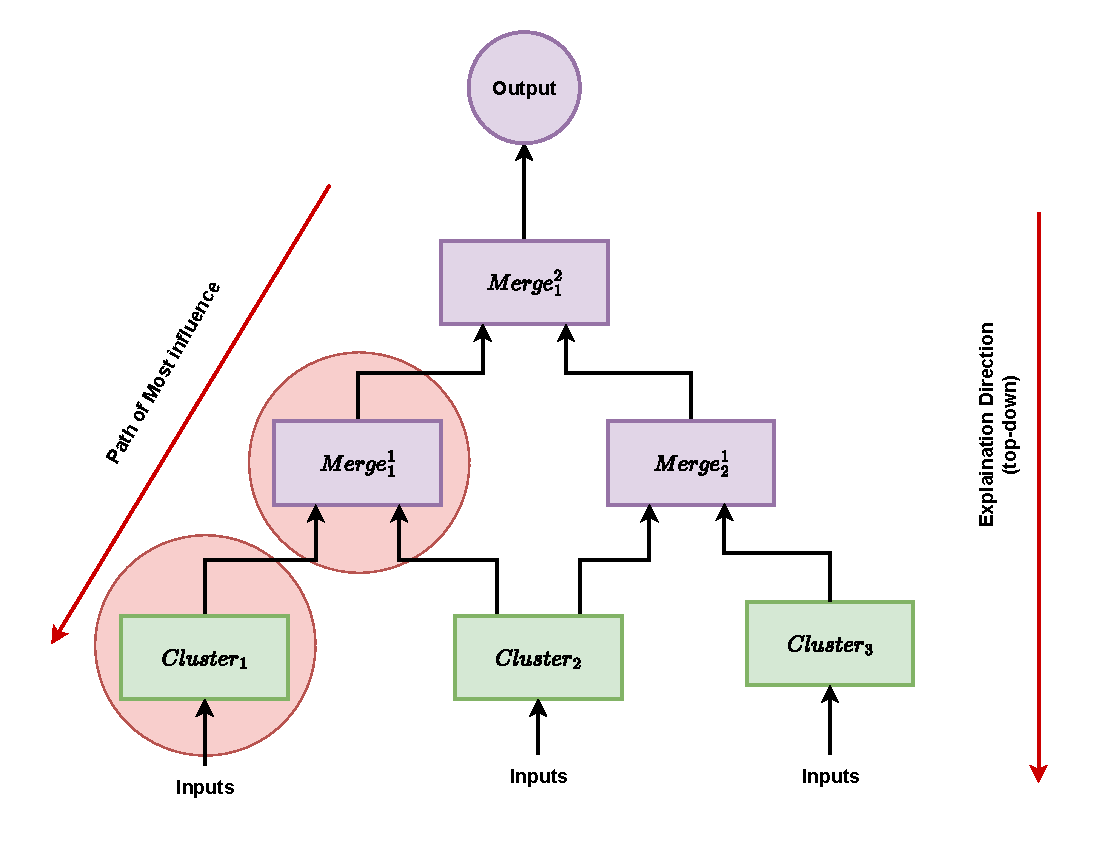
\includegraphics[width=\linewidth]{depression/fig/Shah_explanation_compositional.pdf}
    \caption{Compositional Explainability Methodology}
    \label{fig:comp_explain}
\end{figure}

Using the aforementioned explainability methods is trivial for monolithic/single models. However, the use of compositional models, where we have several sub-models, makes the process of explaining model predictions difficult. While there are various ways of interpreting all possible combinations of cluster models, merge models and combinations of cluster models, we present an intuitive top-down approach.

In our approach, we begin with the Merge model closest to the output and use SHAP values to find the most influential model in the previous stage. We continue this until we reach a cluster model. Using SHAP analysis on the cluster model will provide us with the best input features. The calculation of SHAP differs between classification and regression models, as the number of outputs differs. For a regression model, we simply use the SHAP value we obtain for an instance, as it only produces one output. However, for a classification model which produces $C$ outputs (where $C$ is the number of classes, which is seven in the personalised mood score prediction dataset), we find the mean of the absolute value of the SHAP for the classes and use this value as the output SHAP value. 

For the model in Figure \ref{fig:comp_explain}, we start with $Merge_1^2$. We compute using SHAP that the output from the model $Merge_1^1$ is the most influential. We discover that the output from the model $Cluster_1$ is the most influential for  $Merge_1^1$. Then, we proceed to apply SHAP on this cluster model to obtain the most influential features. ALE plots and Anchor rules\footnote{As Anchors only work with classification models, we used the algorithm defined in Appendix \ref{app:anchors} to extend anchors and explain the predictions of the regression models.}  can also be computed in a similar fashion after the SHAP values and the most influential output/feature have been computed. This approach is beneficial in the case where the number of input features is significant, as it helps focus directly on the most important feature cluster.

The benefit of a compositional model and the explainability method presented is that it allows us to reason about mood score prediction in a hierarchical fashion. We can reason about the outputs of the cluster models and the various merge models. We can also reason about the outputs of combinations of cluster models. For the mood score prediction problem, where we have 43 features as input, the compositional model and the top-down explainability approach help converge on a narrower set of important clusters/models and features faster while ensuring that the effect of feature correlations is mitigated when using SHAP and other explainability methods. 

Furthermore, we can compute the best clusters and models at the population level by following the same top-down approach. For each participant, we hierarchically find the best merge or cluster model in the preceding stage, starting from the output using SHAP. Once found, we sort these models based on their frequency of appearance over the population to find the best overall models at each stage. While most influential features can also be obtained from a monolithic model, these feature influence values will be affected by the interactions between all features considered. A compositional architecture removes some of these interactions through its hierarchical and separated model architecture.

Note that the architecture of the compositional model allows a user to apply explainability methods on any cluster/merge model and analyse the results. Also, we do not compute the SHAP and other explanations on the complete compositional model, as the influence of input feature perturbations or gradient (which is used by most post-hoc explainability methods) will be reduced (almost negligible) due to the hierarchical structure of the compositional model, and hence, such an approach will produce spurious feature importances.




\section{Results}   
\label{sec:depression_results}

In this section, we report the performance and explainability of monolithic and compositional models. We begin with monolithic results and continue with compositional results and comparisons, where applicable. A discussion subsection at the end interprets these findings. Overall, the monolithic results show how MLP models outperform common baseline ML models for several participants, and the compositional results show where decomposition further improves predictive performance and explainability.

\subsection{Monolithic Model Results}

In this section, we report the results of the best base models and the overall best MLP models, computed as discussed in Section \ref{sec:monolithic_model_evaluation}. As we build personalised models, we report each participant's results separately. We present the mean and standard deviation of the \gls{mae} for the best models. Finally, we show the SHAP values, the ALE plots, and the Anchor rules for the participant MLP models.



\begin{table}[htbp]
 \caption{Metrics for the best base and MLP models for each participant. The values in bold indicate lower MAE. (MAE: Mean Absolute Error; STD: standard deviation of MAE; P-1 to P-29 refer to participants 1 to 29.)}
 \centering
 \begin{tabular}{ccc c c}
 \hline
 \multirow{2}{*}{Participant ID} & Model & \multicolumn{2}{c}{MAE} \\
 \cline{3-4}
 &  & Mean & STD \\
 \hline

 \multirow{2}{*}{P-1} 
 & Support Vector Classifier & 0.336 & 0.145 \\
 & MLP Classifier              & \textbf{0.295} & \textbf{0.151} \\
 \hline

 \multirow{2}{*}{P-10} 
 & Random Forest Classifier    & \textbf{0.697} & 0.113 \\
 & MLP Classifier              & 0.715 & \textbf{0.089} \\
 \hline

 \multirow{2}{*}{P-12} 
 & Support Vector Classifier   & \textbf{0.575} & 0.077 \\
 & MLP Regressor               & 0.582 & \textbf{0.063} \\
 \hline

 \multirow{2}{*}{P-14} 
 & Support Vector Classifier   & 0.904 & \textbf{0.146} \\
 & MLP Regressor               & \textbf{0.829} & 0.327 \\
 \hline

 \multirow{2}{*}{P-15} 
 & Gradient Boosting Regressor & \textbf{0.467} & 0.115 \\
 & MLP Regressor               & 0.494 & \textbf{0.050} \\
 \hline

 \multirow{2}{*}{P-18} 
 & Random Forest Classifier    & 0.823 & \textbf{0.185} \\
 & MLP Classifier              & \textbf{0.638} & 0.472 \\
 \hline

 \multirow{2}{*}{P-19} 
 & Gradient Boosting Regressor & 1.072 & 0.171 \\
 & MLP Classifier              & \textbf{0.989} & \textbf{0.096} \\
 \hline

 \multirow{2}{*}{P-20} 
 & Random Forest Classifier    & 0.636 & \textbf{0.181} \\
 & MLP Classifier              & \textbf{0.455} & 0.249 \\
 \hline

 \multirow{2}{*}{P-21} 
 & Random Forest Classifier    & 1.152 & 0.298 \\
 & MLP Regressor               & \textbf{1.103} & \textbf{0.216} \\
 \hline

 \multirow{2}{*}{P-23} 
 & Gradient Boosting Regressor & \textbf{0.883} & \textbf{0.307} \\
 & MLP Classifier              & 0.936 & 0.550 \\
 \hline

 \multirow{2}{*}{P-24} 
 & Support Vector Classifier   & 0.158 & \textbf{0.074} \\
 & MLP Classifier              & \textbf{0.125} & 0.088 \\
 \hline

 \multirow{2}{*}{P-26} 
 & Gradient Boosting Regressor & 1.098 & 0.213 \\
 & MLP Regressor               & \textbf{1.013} & \textbf{0.149} \\
 \hline

 \multirow{2}{*}{P-28} 
 & Random Forest Classifier    & 0.609 & 0.173 \\
 & MLP Classifier              & \textbf{0.562} & \textbf{0.163} \\
 \hline

 \multirow{2}{*}{P-29} 
 &  \gls{adaboost} Regressor          & 1.188 & 0.310 \\
 & MLP Classifier              & \textbf{1.030} & \textbf{0.253} \\
 \hline
 \end{tabular}
 \label{tab:overall_res}
\end{table}



\subsubsection{Model performance}

The best MLP model obtained after optimisation is compared to the best base model for each participant. Table \ref{tab:overall_res} shows the average \gls{mae} values and their standard deviations (MAE STD) for the best base and MLP models evaluated on the 5-fold cross-validation test sets. All models in Table \ref{tab:overall_res} have an MAE of less than or equal to 1, which implies that the difference between the actual mood score and the one predicted is, on average, around 1. 

Moreover, the performance (MAE) of the MLP models is better (lower MAE) than the base models for 10 out of 14 participants, as evidenced by the bold values in Table  \ref{tab:overall_res}. Although the model hyperparameter search methodology differs between the MLP and the base models, the comparison indicates how powerful MLP models (a comparatively simple DL method) are at learning meaningful representations for mood scores from digital data. Also, the disparity in model type and performance can be attributed to the differences in the participant datasets used to build the personalised models. Most participant datasets have missing data and high data imbalance (a higher proportion of a specific mood score), and depending on the type of imbalance and the amount of good data available, it can make it difficult or easier for certain models to learn associations from them. Overall, MLP models seem to be better able to learn the representations between the input features and the mood score.

Furthermore, Tables \ref{tab:best_model_combination} and \ref{tab:best_model_parameters} show hyperparameter combinations and model parameters for the best MLP models reported in Table \ref{tab:overall_res}. We find that Deletion and Manual Imputation are the best methods for handling missing data for the participants used in the study. Also, classification models seem to outperform regression models for both the base and MLP models. Of the 14 best MLP models, 9 are classification models, and 5 are regression models. Moreover, among the optimisers used to optimise the hyperparameters, Bayesian, DE, and PSO are the best methods. There is no visible correlation between the model type, choice of hyperparameters and architecture among the participants, and it seems to be dependent on the participant and the type of model. Appendices \ref{sec:mlp_hyperparameters} and \ref{sec:base_hyperparameters} contain more information on the model hyperparameters and architectures used for the best models. 

 


\subsubsection{MLP model explanation}

\underline{\textit{SHAP explanation}}:


\begin{figure}[htbp]
 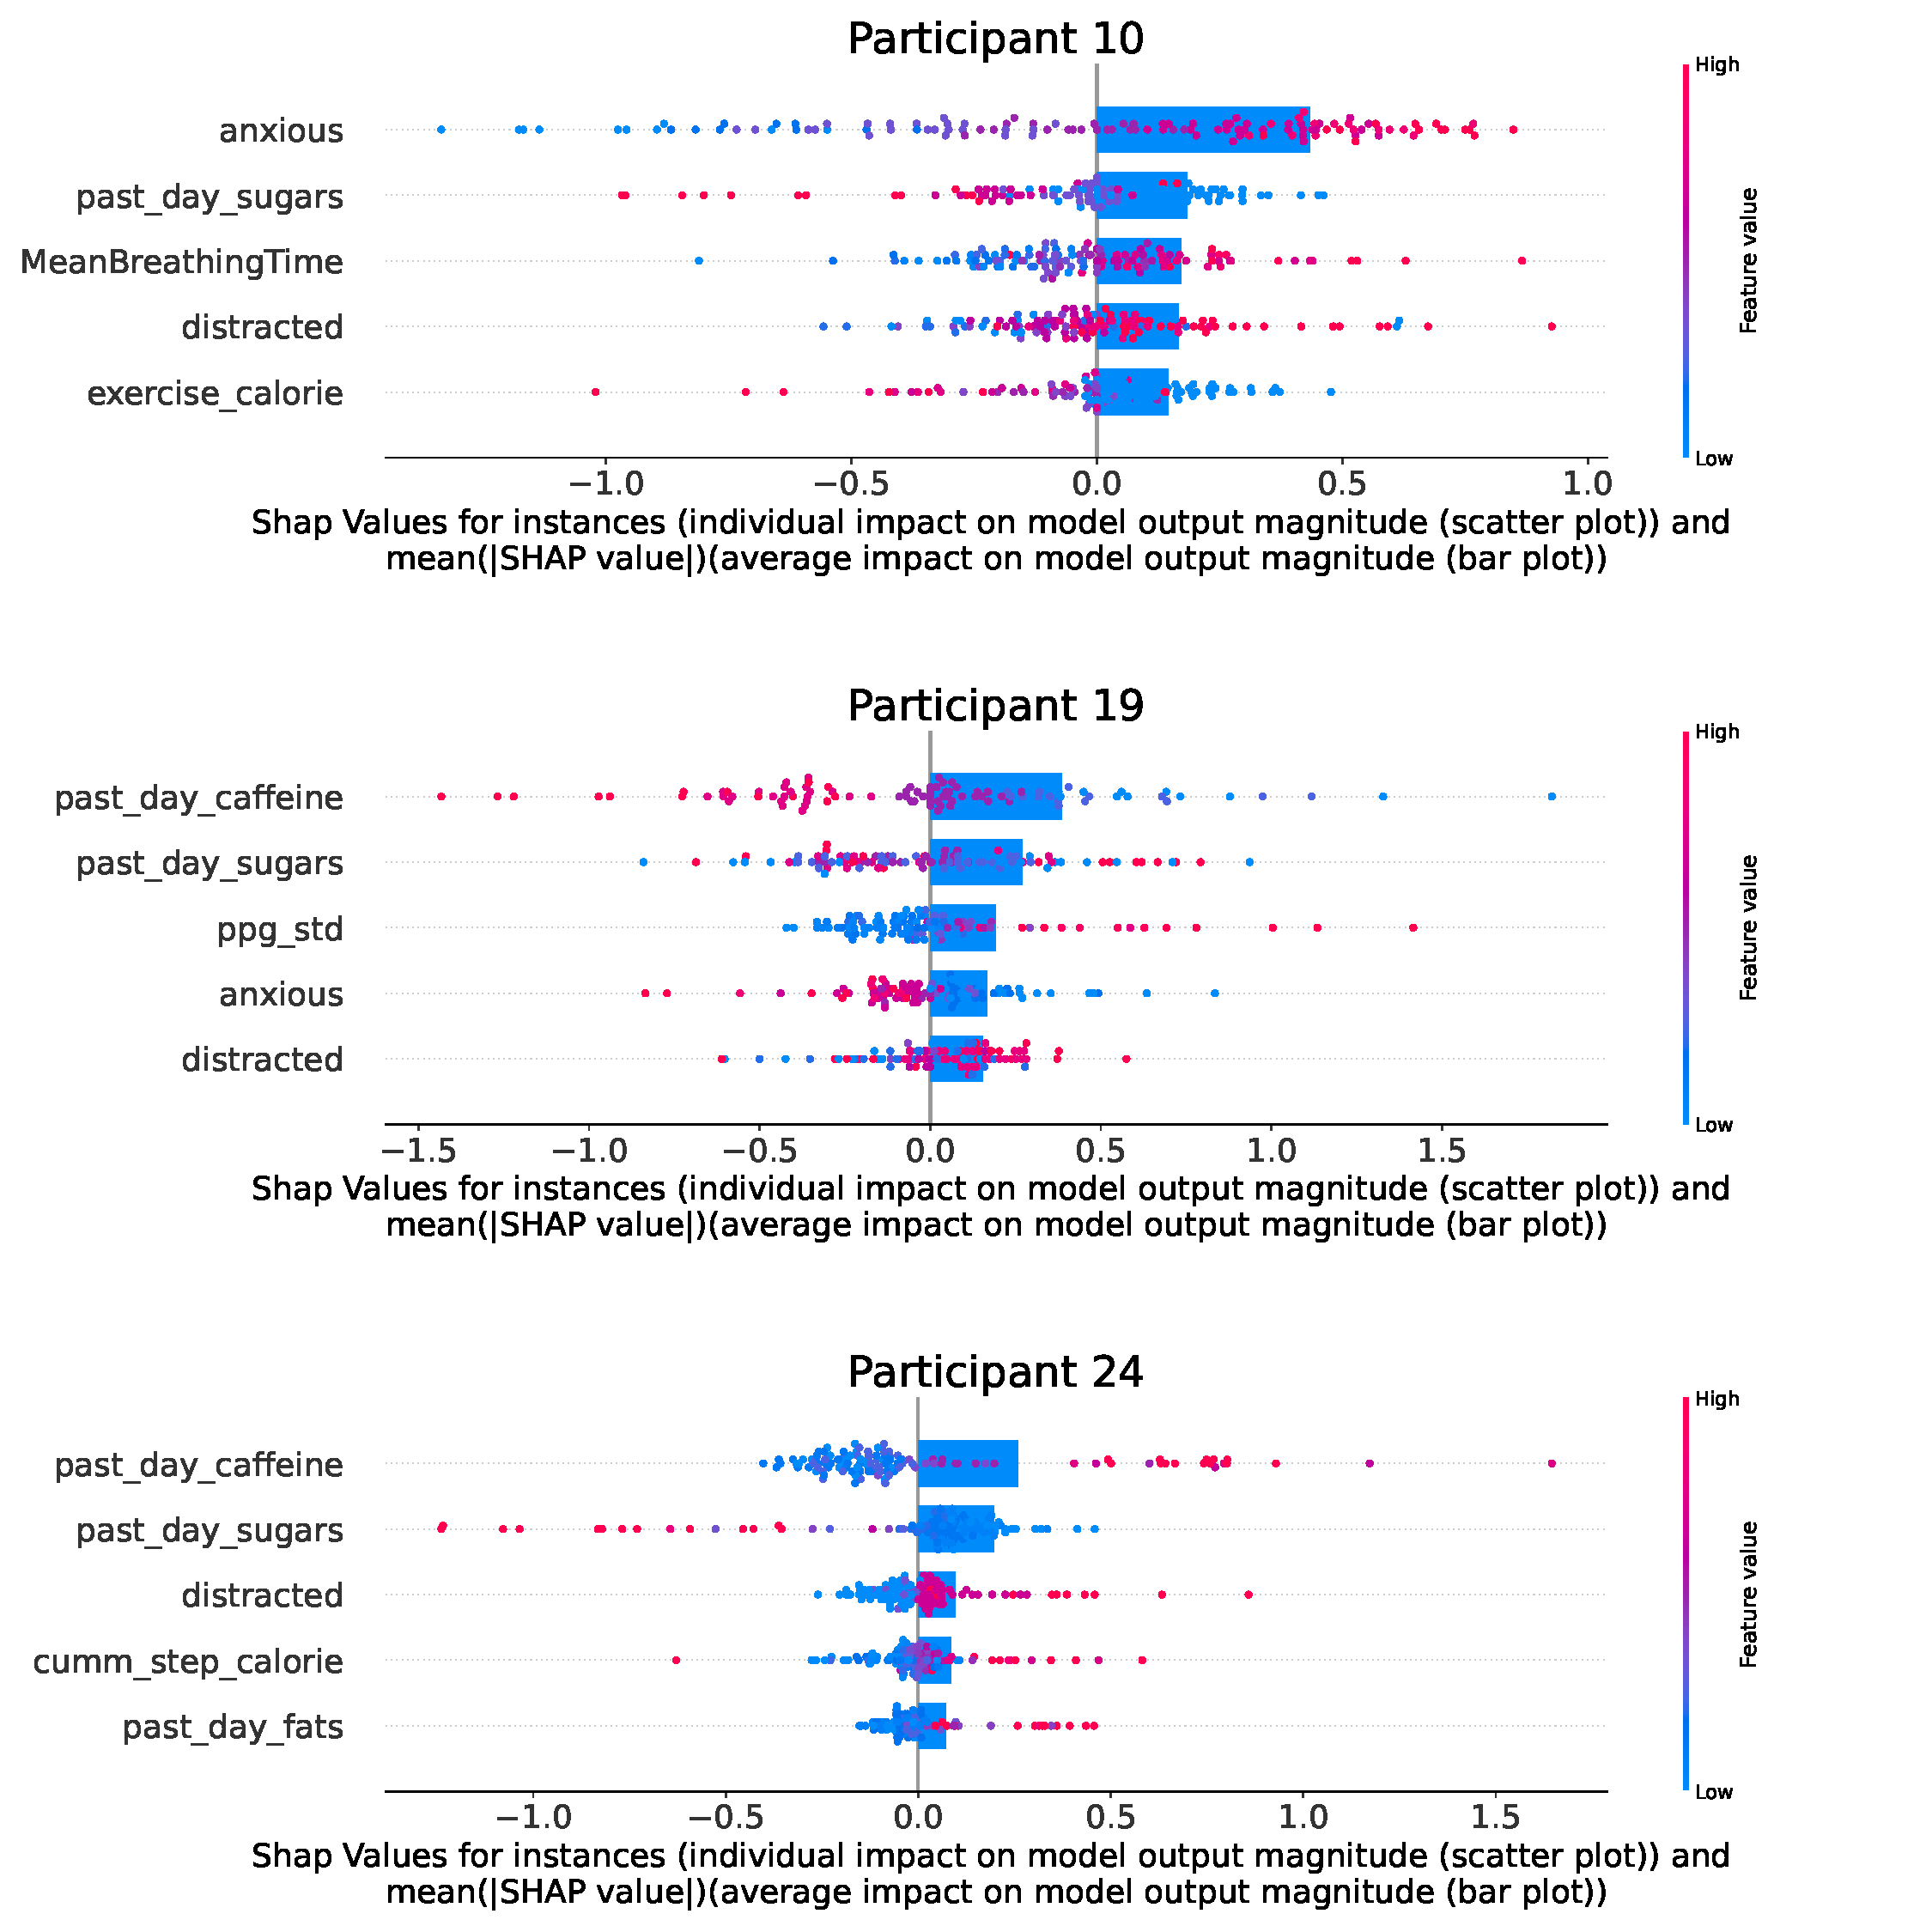
\includegraphics[width = \linewidth]{depression/fig/SHAPOverall_3.pdf}
 \caption{The figure shows the SHAP value effects for the top 5 features in the overall best models for Participants 10, 19 and 24. The scatter plots depict the SHAP values for individual samples, with the colour of the points denoting their magnitude. The bar plots superimposed on top show the mean of the absolute value of the SHAP values over all data points. The features are arranged based on the magnitude of the average SHAP values. Plots for all participants can be found in the appendices.}
 \label{fig:shap_overall}
\end{figure}



\begin{figure}[htbp]
\centering
\begin{subfigure}{0.48\linewidth}
 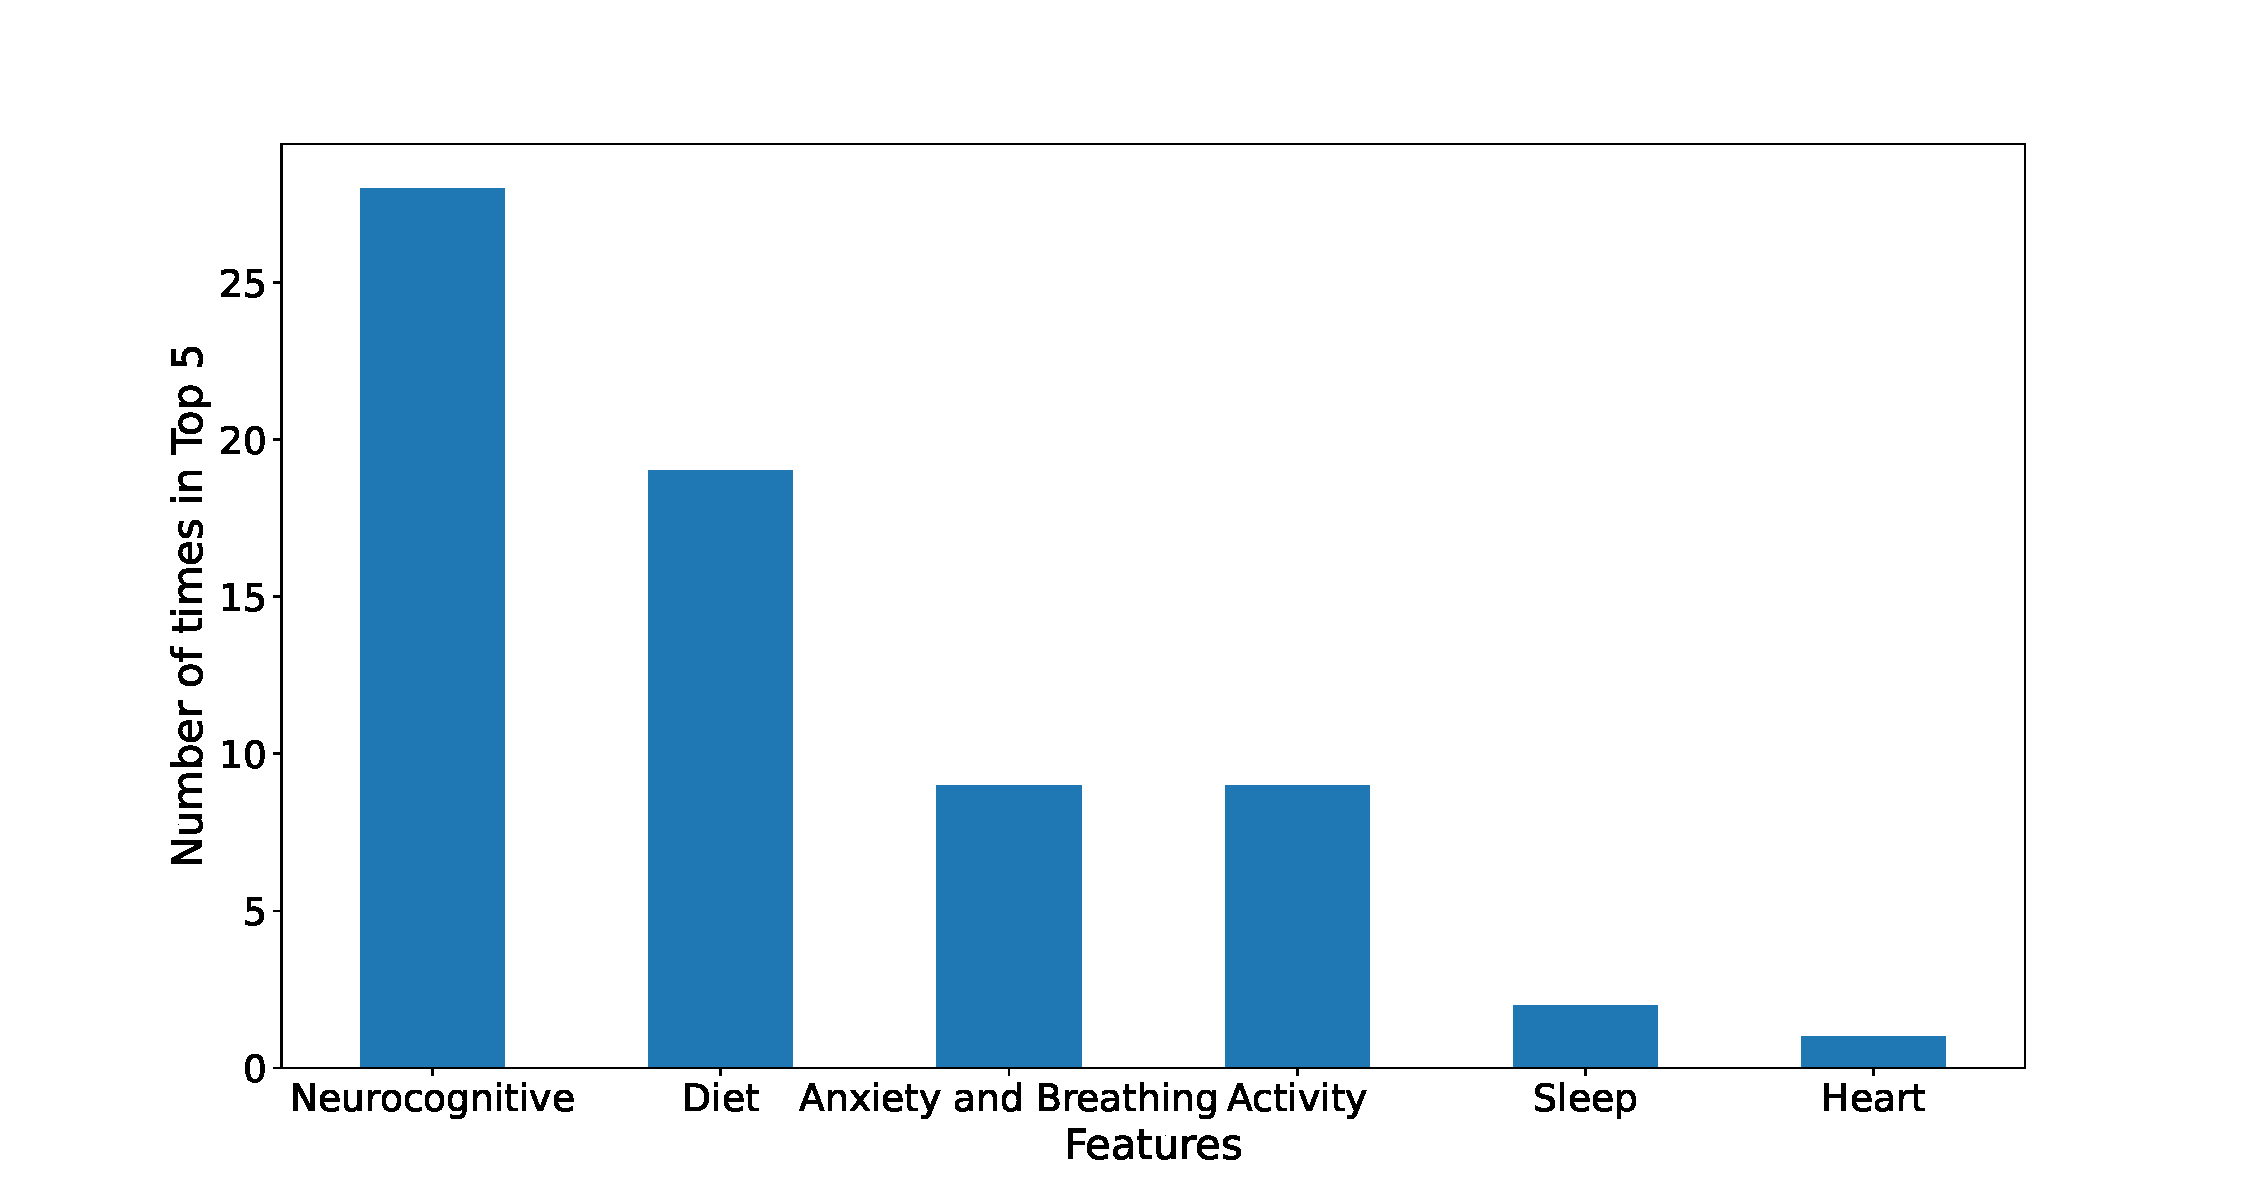
\includegraphics[width=\linewidth]{depression/fig/SHAPOverall_all_neuro_grouped.pdf}
 \caption{Top feature groups in the overall best models for all participants with neurocognitive features.}
 \label{fig:shap_overall_all_sub_neuro}
\end{subfigure}
\hfill
\begin{subfigure}{0.48\linewidth}
 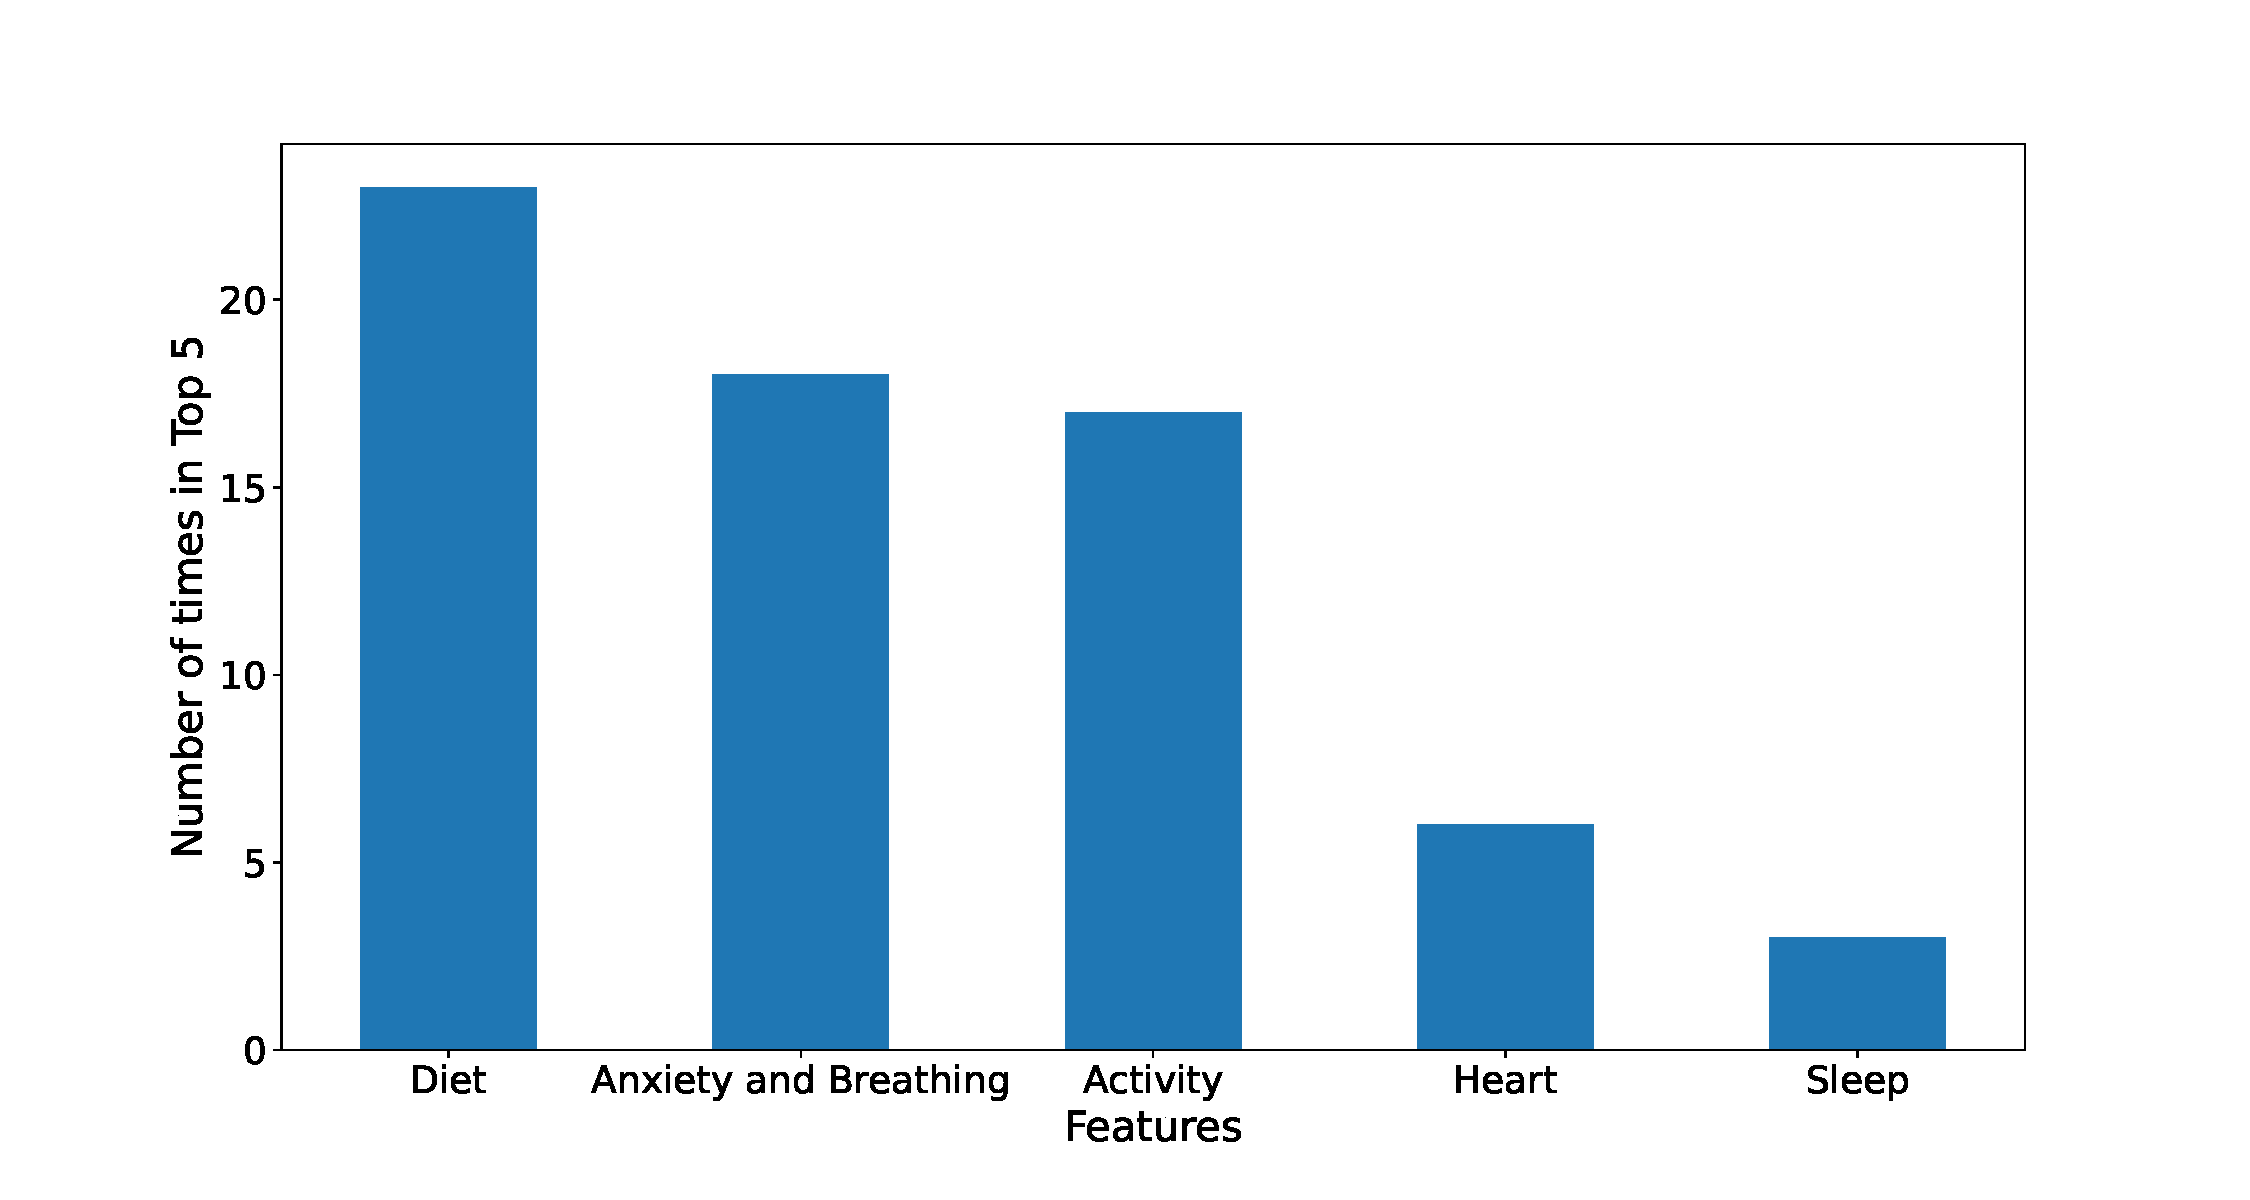
\includegraphics[width=\linewidth]{depression/fig/SHAPOverall_all_grouped.pdf}
 \caption{Top feature groups in the overall best models for all participants without neurocognitive features.}
 \label{fig:shap_overall_all_sub}
\end{subfigure}

\vspace{0.5em}

\begin{subfigure}{0.98\linewidth}
 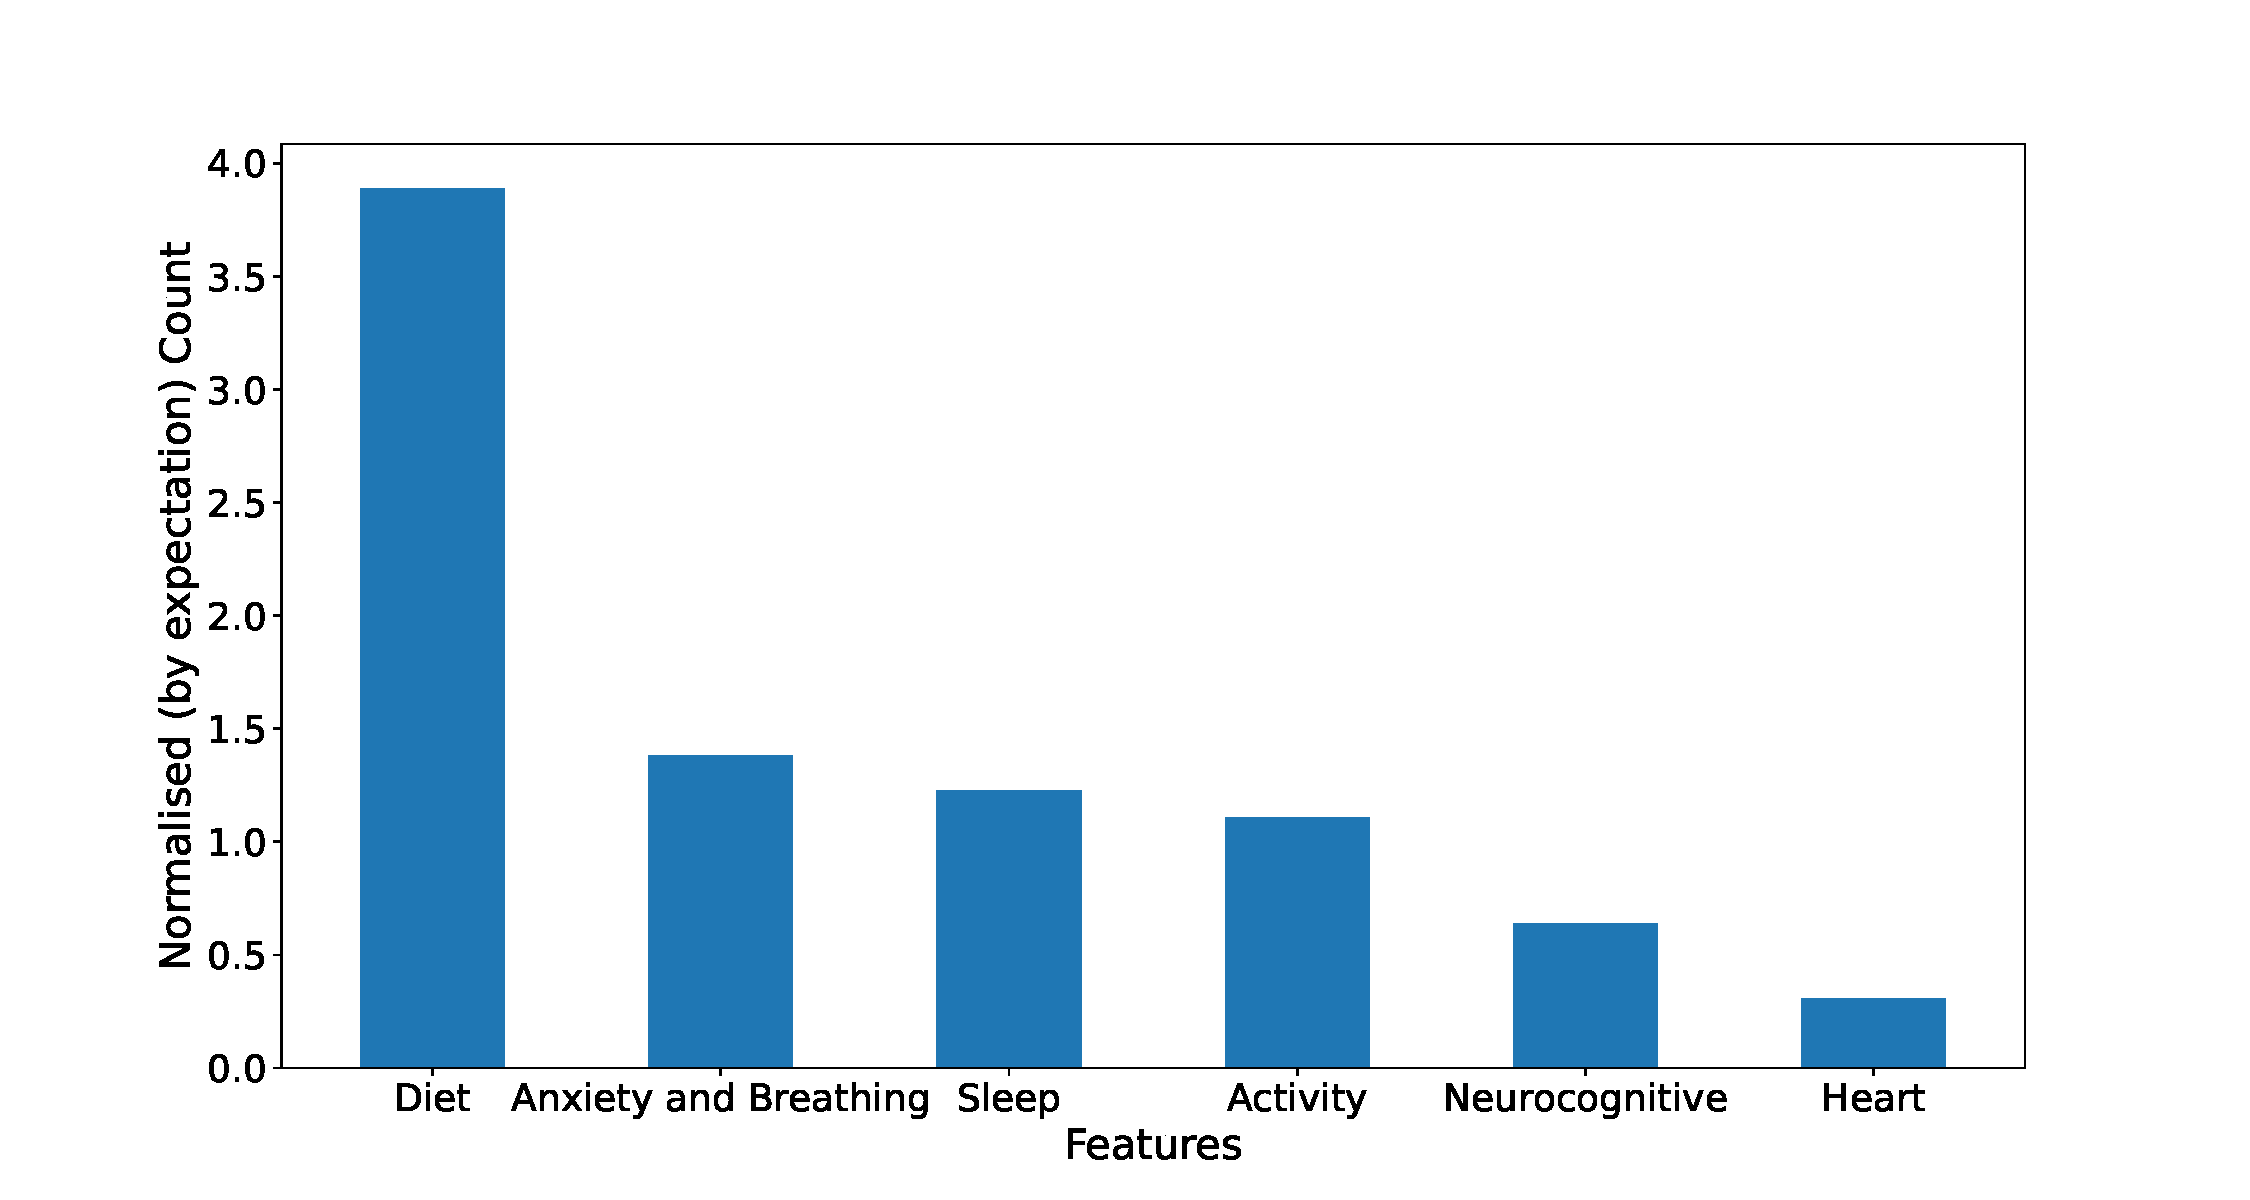
\includegraphics[width=\linewidth]{depression/fig/SHAPOverall_all_grouped_norm_expected.pdf}
 \caption{Top feature groups in the overall best models for all participants with neurocognitive features and corrected for the number of features in each group.}
 \label{fig:shap_overall_all_sub_expected}
\end{subfigure}
\caption{The figure shows the top-5 feature groups in the overall best models for all participants. The features are arranged based on the frequency of their appearance in the top-5 features. The groups contain the following features. Diet: \emph{past-day-fats, past-day-sugars, past-day-caffeine}; Anxiety and Breathing: \emph{anxious, distracted, MeanBreathingTime, Consistency}; Activity: \emph{cumm-step-count, cumm-step-calorie, cumm-step-distance, exercise-calorie, exercise-duration}; Heart: \emph{heart-rate,ppg-std}; Sleep: \emph{prev-night-sleep}; and Neurocognitive: all neurocognitive features.}
\label{fig:shap_overall_all}
\end{figure}



Figure \ref{fig:shap_overall} shows the five features from the wearable- and EMA-acquired features that affect the model prediction most based on their SHAP values for three example participants. Plots for all participants can be found in Appendix \ref{sec:additional_results}. SHAP explains a prediction (a single prediction) of a data instance by computing the contribution of each feature to the prediction. We take the mean (average) of the absolute SHAP values for all instances in the dataset and sort them to find the top 5 features in the figure. 

Figure \ref{fig:shap_overall_all} further shows the overall (population-level or for all participants) top feature groups ranked by the number of times they appear in the top-5 features, i.e. by their frequency, with and without the neurocognitive features and corrected for the number of features in each group. The figure \ref{fig:shap_overall_all_sub_expected} shows that diet-related features, such as \emph{past-day-sugars}, \emph{past-day-fats}, \emph{past-day-caffeine}, have the highest effect on mood score prediction. This is followed by anxiety-based features (measured through features like \emph{anxious}, \emph{distracted}, and \emph{MeanBreathingTime}). As the neurocognitive group contains a large number of features, the uncorrected top feature groups are dominated by neurocognitive features (see Figure \ref{fig:shap_overall_all_sub_neuro}). This analysis shows that the normalisation method and the way we group the features can have a significant impact on the top feature groups.

Furthermore, the scatter plot in the figure shows the SHAP value (effect on mood score) for different feature values. There is variability in how certain features affect mood score prediction. For instance, for Participant 10, low values for the feature \emph{anxious} (see blue dots for Participant 10 in Figure \ref{fig:shap_overall}) lead to a decrease in model prediction by 1 in some instances. Therefore, ensuring lower anxiety for this participant could be a suitable intervention. For instance, an increase in \emph{past-day-caffeine} decreases mood score prediction for Participant 19, whereas the opposite is seen for Participant 24.



\underline{\textit{ALE plot explanation}}:

Although the scatter plots in the SHAP plots show how high and low values of features affect the model output, they are not good at showing trends. We use ALE plots to see feature trends. Figure \ref{fig:ale_overall} shows the ALE plots for the top-5 non-neurocognitive features obtained from the overall best models using SHAP value analysis. These plots can help a physician understand how the top predictors influence the model prediction (mood score) with their values. While the plots for some features in some participants are quite simple, others are more complex, denoting a heterogeneity in depressive severity and symptoms. The feature effect values (the ALE values) for participants will differ from SHAP, as ALE plots show only the feature effects separated from any correlation effects between the features (which SHAP does not remove). Also, a positive value (or negative value) on the plot signifies an increase (or decrease) in mood score prediction. The ALE value in the plot shows the magnitude of such effects.

Taking the example of Participant 10, the ALE value of high \emph{anxious} and \emph{distracted} is high. This implies that a high value of both features leads to an increase, i.e. an overall increase in mood score (or depression). The effect of features is not consistent across participants and may seem counterintuitive. For instance, for Participant 19, an increase in \emph{past-day-caffeine} (amount of caffeinated items consumed last day) and \emph{past-day-sugars} (amount of sugary items consumed last day) leads to a decrease in mood score (less depressed). This may seem counterintuitive, as having too many sugary food items is generally unhealthy. In such instances, other explainable methods, such as SHAP and Anchors (as discussed later), could be used to increase trust in the plots. Comparing these results to the SHAP plot (see the scatter plots in Figure \ref{fig:shap_overall}) for Participant 19, we see that high values of \emph{past-day-caffeine} and \emph{past-day-sugars} decrease the SHAP value or the model prediction of mood score. As the SHAP explanation aligns with the findings of the ALE plots, it increases our trust in the ALE findings.

Figure \ref{fig:ale_overall} also shows that for some participants, such as participant 24, the feature effect of \emph{distracted} is nearly zero. This does not necessarily mean the feature is unimportant or has no trends. It may happen if one half of the dataset exerts a positive effect and the other half a negative effect, one half cancelling the effect of the other half during averaging. Not much helpful information can be gathered from the plots in such instances. Nevertheless, ALE plots are one of the best for visualising any feature's true effect trends in the presence of interactions/correlation between features.



\begin{figure}[htbp]
 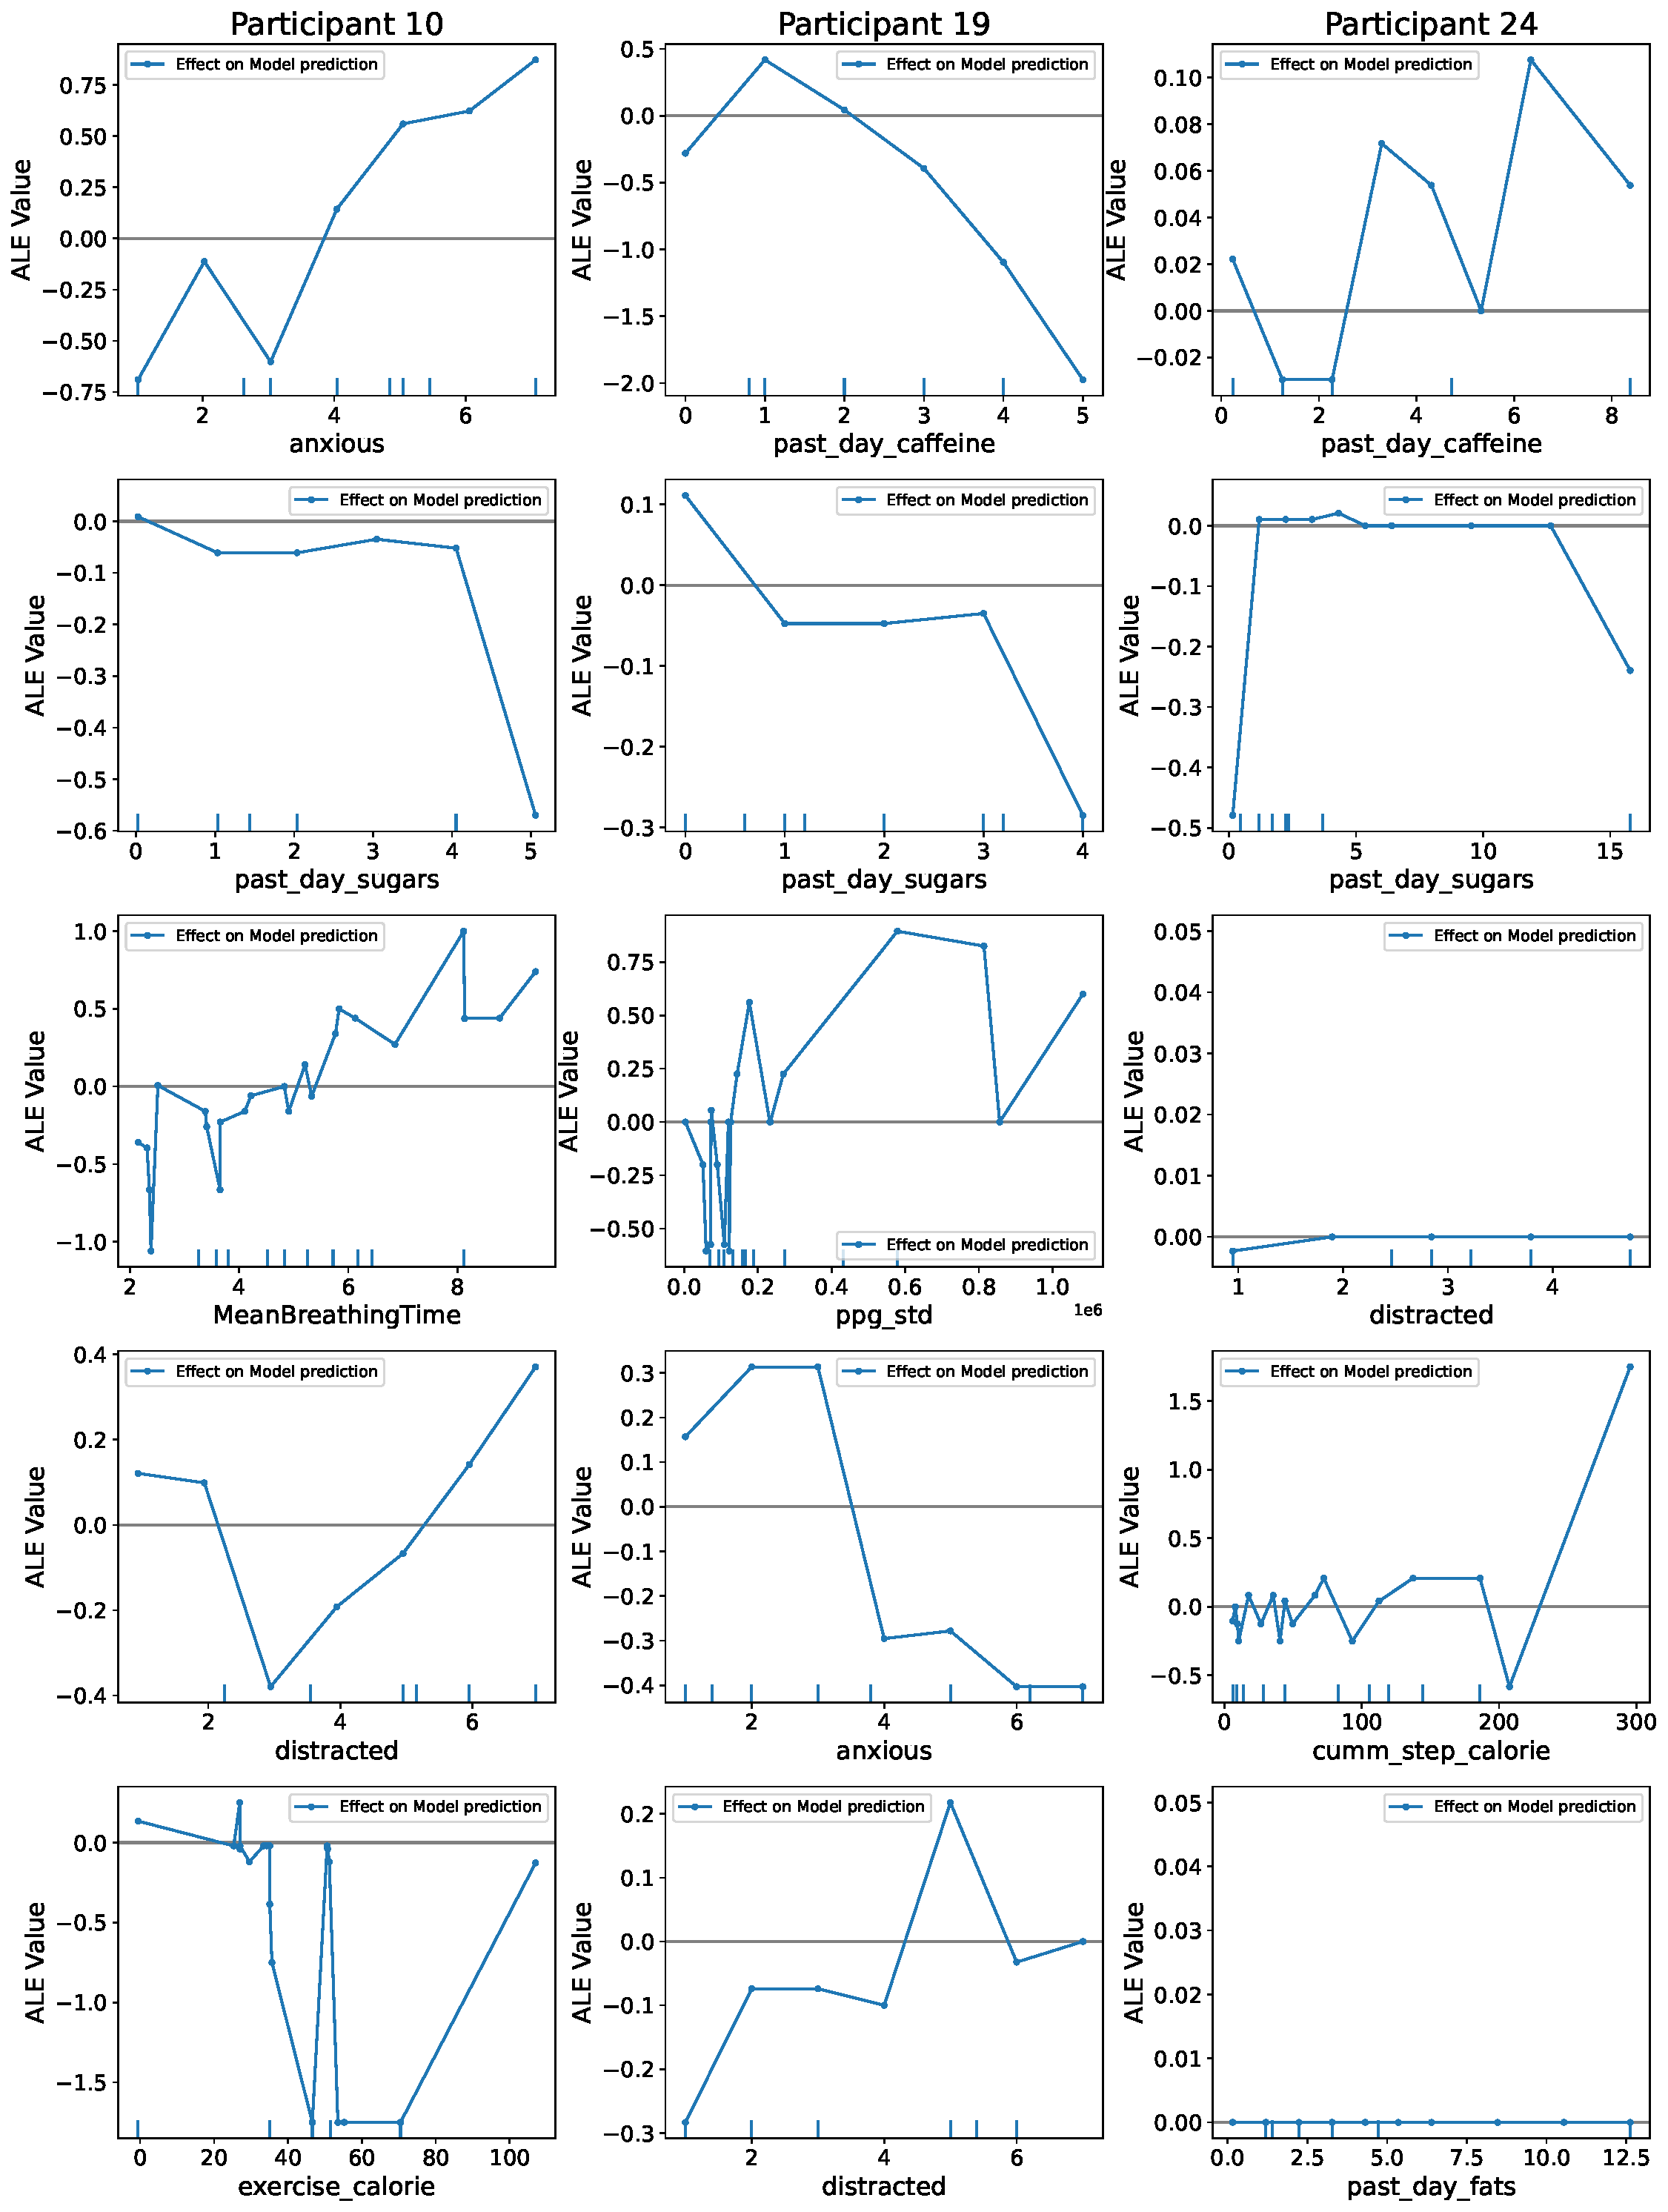
\includegraphics[width = \linewidth]{depression/fig/ALEOverall_argmax_1.pdf}
 \caption{The figure shows the Accumulated Local Effects (ALE) plots for the top-5 features in the overall best models for Participants 10, 19 and 24. The x-axis contains the feature values, and the y-axis contains the ALE values. The ALE values denote the magnitude of the average effect of a feature value on the model output, i.e., the mood score. Plots for all participants can be found in the appendices. }
 \label{fig:ale_overall}
\end{figure}


\underline{\textit{Anchors explanation}}:

Finally, we show how Anchors can explain unusual mood scores by finding the best decision rules (predicated on the features) that apply to a prediction. For instance, a participant's mood score may increase by three points (e.g. from 3 to 6), signifying a sudden increase in a depressive mood. By comparing the IF-THEN-based rules obtained from Anchors before and after such changes, we can surmise what may have changed in the observed features to elicit such a mood change. 

The Anchors procedure takes in a sample corresponding to a mood score prediction, perturbs the sample to create artificial samples in the neighbourhood of the original sample, and finds the region (rules) in the perturbed neighbourhood where the decision rules do not change the prediction. Since this method can only be used for classification models, we use it on participants where the best model is a classification model. Also, we only use it for instances where the prediction was correct to ensure the rules have fidelity.

Also, Anchors allow the user to specify the maximum number of features to use when finding the rules. This allows the user to choose between concise or comprehensive rules. To show how Anchor rules can be constructed and interpreted, we use anomalous instances from Participants 1, 10 and 24. We begin with the case where the mood score for Participant 1 increases from 3 to 5 within 19 hours, and use a maximum of five features to construct the rules.


\begin{multline}
IF \ [(past-day-fats \leq 11.40 \ items) \land (GLbias-dACC > 0.00)] \ THEN; \\
Depressed = 3 \\
Precision: 1\\
Coverage: 0.20 \\
\\
IF \ [(past-day-sugars > 25.00 \ items) \land (distracted > 5.00) \land (cumm-step-calorie \leq 285.62)] \\ THEN;
Depressed = 5 \\
Precision: 0.95\\
Coverage: 0.03 \\
 \label{eq:ucsd1}
\end{multline}

Equation \ref{eq:ucsd1} shows the conditions/rules on the features needed to ensure that the mood score prediction (\emph{Depressed} in the equation) changes from 3 to 5, where $GLbias-dACC$ is the neural activity in the dACC brain region corresponding to bias for frequent gains (see the appendices section in \cite{shah_personalized_2021}). The first set of conditions pertains to the case when the mood score is 3, and the second set is when the score is 5. 

Furthermore, the Precision and Coverage values in the Anchors in Equation \ref{eq:ucsd1} say that the anchors applied to 20\% (3\% (in the second set of conditions)) of the perturbation space instances and 100\% (95\%) of those instances conformed to the rule, i.e. had a prediction of 3 (5). Higher precision and coverage imply greater fidelity of anchor rules to the model behaviour. If we compare the Anchors, we observe that less physical activity, being more distracted and consuming significant amounts of sugary food items (more than 25) are associated with a high mood score/depressive mood. Also, it appears that having fewer fatty food items helps keep the mood score (depression) moderately low (at 3). 

Although Anchor rules provide good human-readable explanations for instances, it may be difficult to find rules if the maximum number of features chosen to construct the rules is insufficient. Also, finding more Anchors around the change and future changes should provide a good idea of what feature variations lead to a change in mood score. A similar strategy can also be adopted for other participants to explain normal instances. We could also extend the use of Anchors to describe a period of unusual mood scores by explaining all instances within the period and finding the common rules within the instances. A similar analysis can be obtained for participants not presented here.

\subsection{Compositional Results}\label{sec:depression_compositional_results}
In this section, we present the performance comparison results between the monolithic and compositional personalised mood score prediction models, their performance obtained as discussed in Section \ref{sec:monolithic_model_training}. We follow this with a deep dive into how compositional designs can aid explanation using SHAP, ALE plots and Anchor rules, and a comparison of clinical interpretability with monolithic models.

\subsubsection{Model Performance}


\begin{table}[htbp]
 \caption{Table containing the metrics for the best monolithic and compositional MLP models for each participant and the compositional approach. The values in bold indicate lower values. (MAE: Mean Absolute Error; STD: standard deviation of MAE; P-1 to P-29 refer to participants 1 to 29.)}
 \label{tab:performance_comparison}

 \begin{tabular}{cccccccc}
 \hline
 \multirow{2}{*}{ID} & Model & \multicolumn{2}{c}{MAE} & \multirow{2}{*}{ID} & Model & \multicolumn{2}{c}{MAE} \\
 \cmidrule(r){3-4} 
 \cmidrule(r){7-8} 
 &  & Mean & STD & &  & Mean & STD  \\
 \hline

 \multirow{3}{*}{P-1}  & Monolithic &\textbf{ 0.295} & 0.151 &
 \multirow{3}{*}{P-10}   & Monolithic & 0.715 & \textbf{0.089} \\
 & Approach 1 & 0.327 & 0.087  & 
 & Approach 1 & 0.778 & 0.161 \\
 & Approach 2 & 0.345 & 0.1 & 
 & Approach 2 & \textbf{0.673 }& 0.098 \\
 & Approach 3 & 0.361 &\textbf{ 0.086} & 
 & Approach 3 & 0.695 & 0.139 \\
 \hline
 \multirow{3}{*}{P-12}  & Monolithic & 0.582 & 0.063 & 
 \multirow{3}{*}{P-14}  & Monolithic & 0.829 & 0.327  \\
 & Approach 1 & \textbf{0.565} & 0.072 &
 & Approach 1 & 0.876 & 0.349  \\
 & Approach 2 & 0.577 & 0.053 & 
 & Approach 2 & 0.83 & 0.426 \\
 & Approach 3 & 0.617 & \textbf{0.044} & 
 & Approach 3 & \textbf{0.814} & \textbf{0.179} \\
 \hline

 \multirow{3}{*}{P-15}  & Monolithic & 0.494 & \textbf{0.05} & 
 \multirow{3}{*}{P-18}  & Monolithic & \textbf{0.638} & 0.472  \\
 & Approach 1 & \textbf{0.4} & 0.154 &
 & Approach 1 & 0.686 & 0.409  \\
 & Approach 2 & 0.441 & 0.058 & 
 & Approach 2 & 0.698 & \textbf{0.043} \\
 & Approach 3 & 0.433 & 0.072 & 
 & Approach 3 & 0.67 & 0.167 \\
 \hline


 \multirow{3}{*}{P-19}  & Monolithic & 0.989 & \textbf{0.096} &
 \multirow{3}{*}{P-20}   & Monolithic & \textbf{0.455} & 0.249 \\
 & Approach 1 & 1.005 & 0.157  & 
 & Approach 1 & 0.586 & 0.161 \\
 & Approach 2 & 0.912 & 0.103 & 
 & Approach 2 & 0.495 & \textbf{0.094} \\
 & Approach 3 & \textbf{0.909} & 0.104 & 
 & Approach 3 & 0.492 & 0.126 \\

 \hline
 \multirow{3}{*}{P-21}  & Monolithic & 1.103 & 0.216 & 
 \multirow{3}{*}{P-23}  & Monolithic & 0.936 & 0.55  \\
 & Approach 1 & 1.114 & 0.218 &
 & Approach 1 & 0.872 & 0.291  \\
 & Approach 2 & \textbf{1.012} & \textbf{0.2} & 
 & Approach 2 & 0.865 & 0.319 \\
 & Approach 3 & 1.075 & 0.21 & 
 & Approach 3 & \textbf{0.836} &\textbf{ 0.263} \\
 \hline
 \multirow{3}{*}{P-24}  & Monolithic & 0.125 & 0.088 & 
 \multirow{3}{*}{P-26}  & Monolithic & 1.013 & 0.149  \\
 & Approach 1 & 0.175 & 0.119 &
 & Approach 1 & 1.037 & 0.222  \\
 & Approach 2 & 0.158 & 0.126 & 
 & Approach 2 &\textbf{ 0.96} & \textbf{0.118} \\
 & Approach 3 & \textbf{0.108} & \textbf{0.07} & 
 & Approach 3 & 0.992 & 0.151 \\
 \hline
 \multirow{3}{*}{P-28}  & Monolithic & 0.563 & 0.163 &
 \multirow{3}{*}{P-29}   & Monolithic & 1.03 & 0.253 \\
 & Approach 1 & 0.59 & \textbf{0.156}  & 
 & Approach 1 & 1.146 & \textbf{0.141} \\
 & Approach 2 & \textbf{0.524} & 0.178 & 
 & Approach 2 & \textbf{0.935} & 0.221 \\
 & Approach 3 & 0.619 & 0.276 & 
 & Approach 3 & 0.957 & 0.22 \\
 \hline

\end{tabular}
\label{tab:overall_res1}
\end{table}


We perform a performance comparison between the best models for monolithic and the three compositional MLP-based models obtained after optimisation. Table \ref{tab:performance_comparison} shows the average Mean Absolute Error (MAE) and its standard deviation (MAE STD) of the best MLP models calculated over the five folds of the cross-validation procedure.


We can see from the Table that most models have MAEs less than or equal to 1. Furthermore, the compositional models outperform (have the lowest MAE) the monolithic models\footnote{We only compare with the monolithic models for the best MLP models, as the MLP models were the best models at the population level.} in 11 out of 14 participant models, as evidenced by the bold values in Table \ref{tab:performance_comparison}. Although the optimisation methodology is different for monolithic and compositional models (due to differences in architecture), the results show the strengths of the compositional approach in learning useful representations from mood score data. 

We also observe that the best compositional modelling approach varies between participants. This observation can be attributed to the differences in the participant datasets, the inherent representations, and the choice of clusters used to build the compositional models. Most participant datasets have missing values and significant class imbalance—where one mood score predominates—which, depending on the imbalance type and the quantity of reliable data, can either restrict or facilitate a given model's ability to learn meaningful associations. Also, as previously stated, we did not adequately explore all possible combinations of model architectures and cluster combinations, as our goal is to illustrate the benefits of the compositional approach as a whole, and it may be possible to obtain compositional models that exceed the performance of models reported here.

Moreover, we find that Deletion and Manual Imputation are the best methods for handling missing data for the participants used in the study. Also, regression models seem to outperform classification models for the compositional models, in contrast to the monolithic models. There is also no visible correlation between the model type, choice of hyperparameters and MLP architecture among the participants, and it seems to be dependent on the participant and the type of model. The code used to train the models with all the parameters and hyperparameters will be provided upon request.




\subsubsection{Population-level Importances}


\begin{figure}[htbp]
 \centering
 % Top row: Merge figures
 \begin{subfigure}{0.48\linewidth}
 \centering
 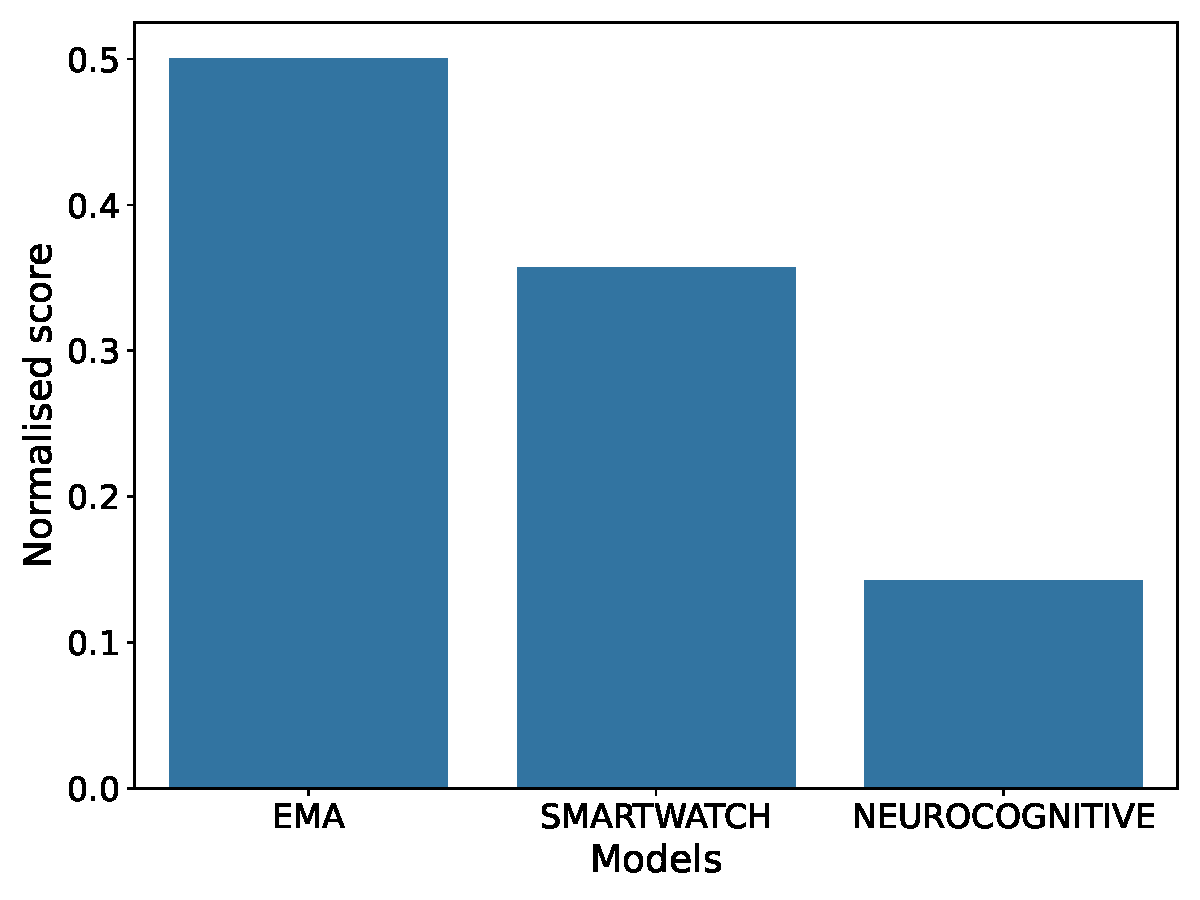
\includegraphics[width=\linewidth]{depression/fig/population_stage2.pdf}
 \caption{Best Stage 2 Merge models at the population level}
 \label{fig:best_pop_1}
 \end{subfigure}
 \hspace{0.5em}
 \begin{subfigure}{0.48\linewidth}
 \centering
 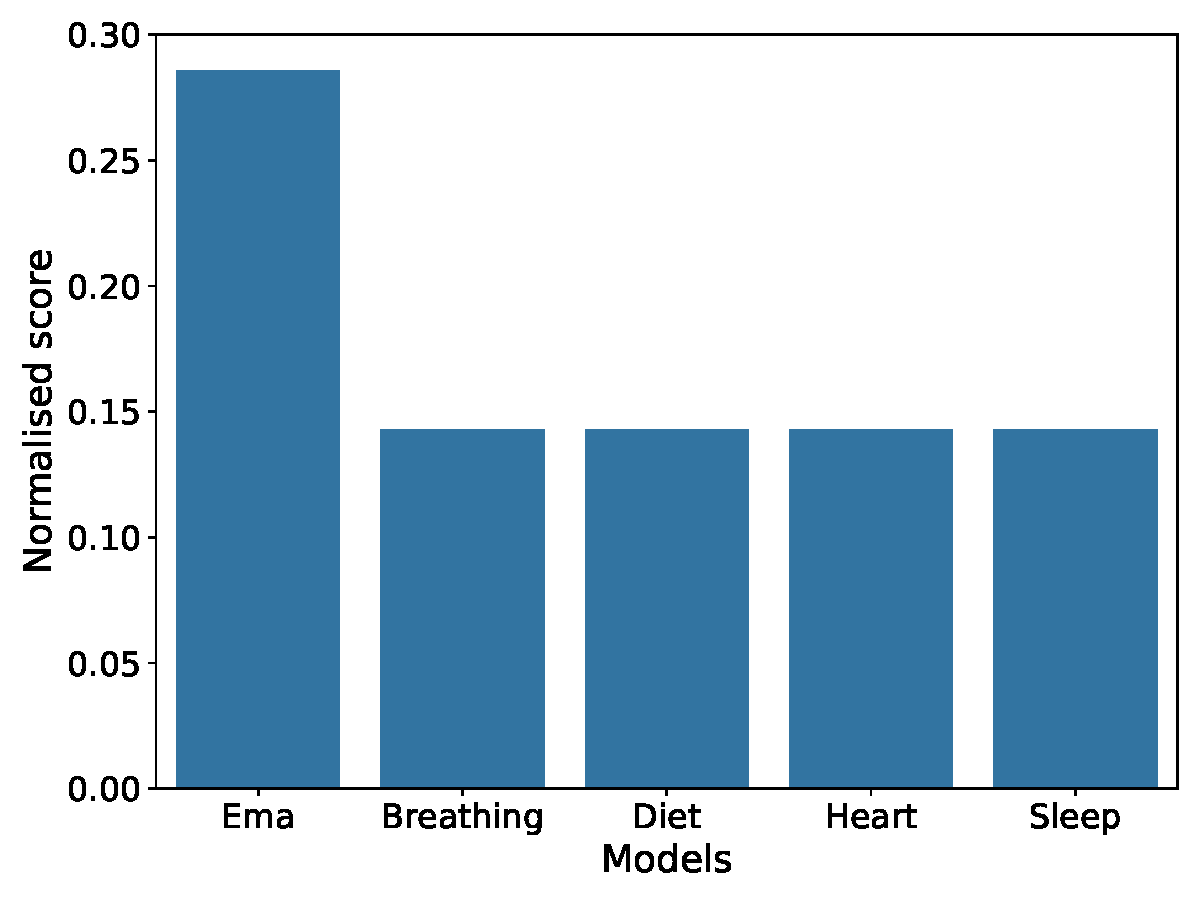
\includegraphics[width=\linewidth]{depression/fig/population_stage1.pdf}
 \caption{Best Stage 1 Merge models at the population level}
 \label{fig:best_pop_2}
 \end{subfigure}
 \caption{Normalised Frequency of Best models at the population level for Approach 3.}
 \label{fig:best_pop}
\end{figure}

We can calculate the best population-level\footnote{By population, we mean the population sample considered in this study and not the general population.} (among 14 participants) cluster and merge models for Participant 19 and Approach 3 using the method mentioned in Section \ref{sec:compositional_model_evaluation}, providing a general overview of the trends. Figure \ref{fig:best_pop} shows the bar plots for the best models. We can see that EMA is the best model for Stage 2 Merge models, followed by Smartwatch and Neurocognitive Merge models. Moreover, Ema, Breathing, and Diet (models that feed into the EMA Merge Model) are the best 3  cluster models at the population level. Also, Breathing, Heart, Diet, and Sleep cluster models have the same importance at the population level.

Thus, we can say that features in the EMA cluster have the most direct and consistent association with mood change. Unfortunately, we cannot perform a direct comparison with the population-level results of \cite{shah_personalized_2021} as the input features in the clusters are different between their study and ours. To see the best models for other approaches, please see Tables \ref{tab:approach1_best_all}, \ref{tab:approach2_best_all}, and \ref{tab:approach3_best_all}. 

Unlike the top feature groups shown in Figure \ref{fig:shap_overall_all} for the monolithic models, the best models for the population level are not affected by the normalisation method. As the compositional models are already built on groups of features (i.e. explicit clustering of features), there is no need to group the features again. This reduces the impact of post-processing steps on the top feature groups, allowing us to obtain population-level insights easily. The only exception is the choice and the number of clusters (during the model design phase), which can affect the top feature groups.



\subsubsection{Compositional Explainability}

Although we can present the explainability results (evaluated using the method in Section \ref{sec:compositional_model_evaluation}) for all participants and their three compositional models, to ensure conciseness, we only present and explain the results when using Approach 3 (the most complex architecture we consider) with Participant 19 to demonstrate the explainability pipeline. A similar analysis can be obtained for other compositional architecture approaches and participants whose results are not presented here. Tables \ref{tab:approach1_best_all}, \ref{tab:approach2_best_all}, and \ref{tab:approach3_best_all} contain the best models for each stage and for all participants when using Approach 1, 2 and 3, respectively. 

We use SHAP to find the top influential/important input features for mood score prediction, use ALE plots to find how the effect of these top input feature values changes with their values, and use anchors to explain individual instances. While we can also look into the top-k, where k is a natural number, input features at each stage of the explanation, we did not present this to ensure brevity.


Approach 3 (presented in Section \ref{sec:compositional_model_architecture}) uses a model with three stages. We start from the Merge model (in stage 3) in Approach 3 and find the most important model feeding into the Merge model (from stage 2) through SHAP, ALE plots and Anchors. We then find the most important cluster model (Stage 1) for the best Stage 2 model. Finally, the best input features for the cluster model are computed. \newline


\underline{\textit{Feature Importances using SHAP:}} 

Figure \ref{fig:shap_ucsd19_approach3} shows the average SHAP values for Participant 19 when using a compositional model developed using Approach 1. Figures \ref{fig:part19_stage2}, \ref{fig:part_19_smartwatch}, and \ref{fig:part_19_heart} show the heatmap plots of the SHAP values averaged over a day.  The top and right axes show the average of the absolute SHAP values over all recorded days and the sum of the average SHAP values over the input features (the inputs going into a Cluster/Merge model), respectively. Similarly, figures  \ref{fig:part19_stage2_summary}, \ref{fig:part_19_smartwatch_summary}, and \ref{fig:part_19_heart_summary} show the SHAP scatter plots showing how the top-5 feature values affect the output mood score prediction.

\begin{figure}[htbp]
 \centering

 % Top row: Merge figures
 \begin{subfigure}{0.48\linewidth}
 \centering
 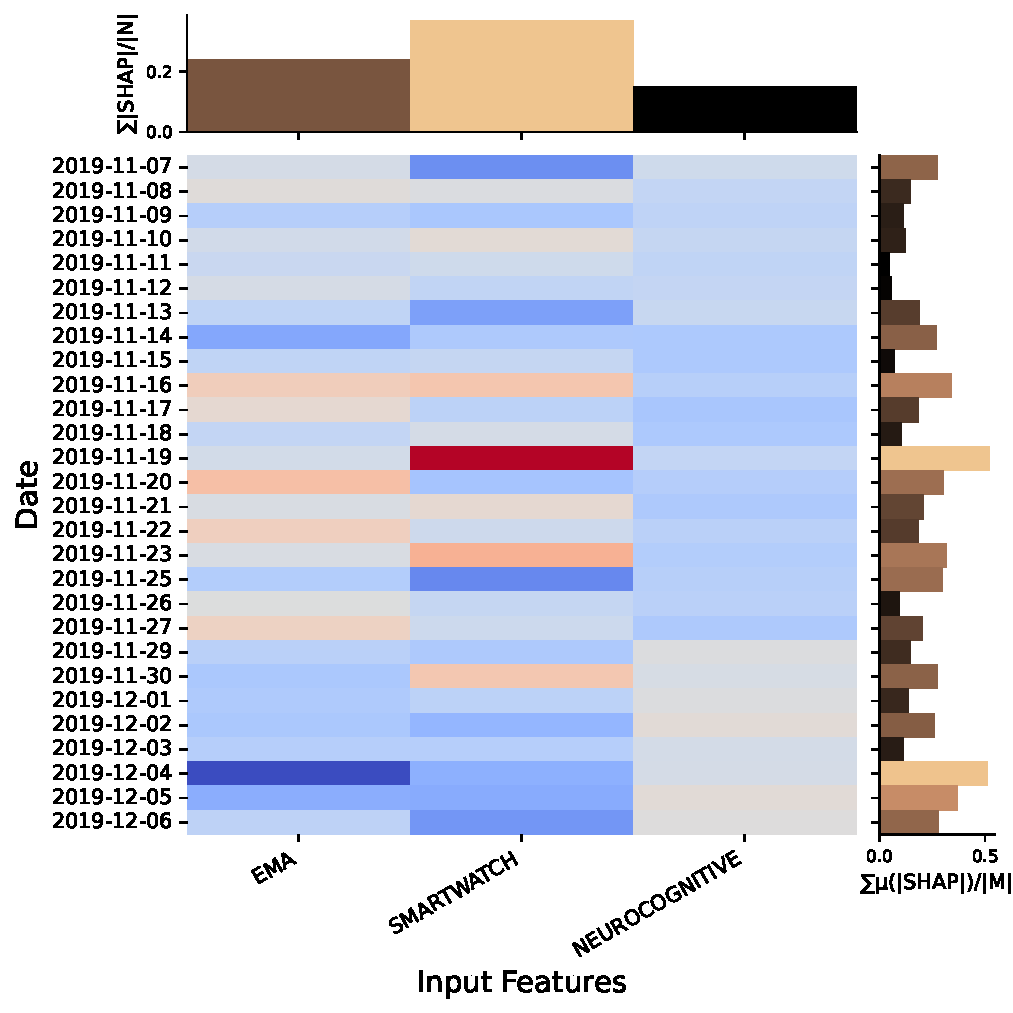
\includegraphics[width=\linewidth]{depression/fig/final_SHAP_comp_Stage2_combined_ucsd19.pdf}
 \caption{SHAP heatmap for the Merge model}
 \label{fig:part19_stage2}
 \end{subfigure}
 \hfill
 \begin{subfigure}{0.48\linewidth}
 \centering
 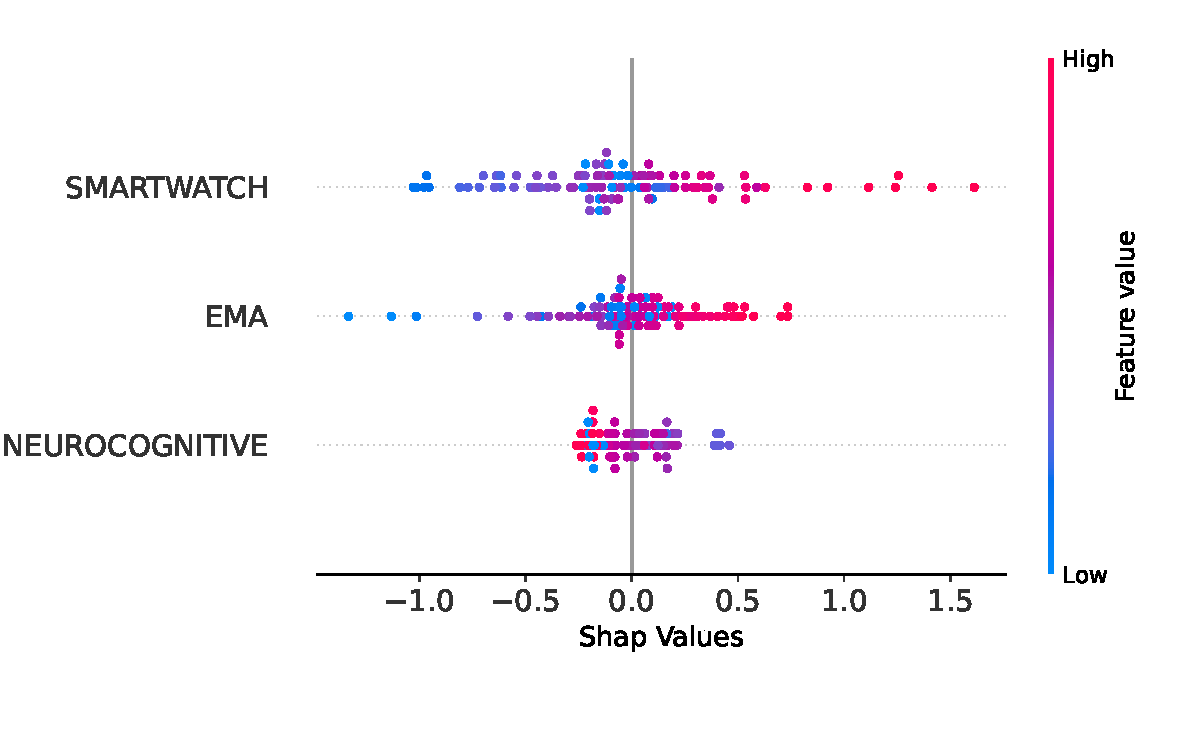
\includegraphics[width=\linewidth]{depression/fig/final_SHAP_summary_comp_Stage2_combined_ucsd19.pdf}
 \caption{SHAP summary for the Merge model}
 \label{fig:part19_stage2_summary}
 \end{subfigure}

 \vspace{0.5em} % Optional spacing between rows

 % Bottom row: Food figures
 \begin{subfigure}{0.48\linewidth}
 \centering
 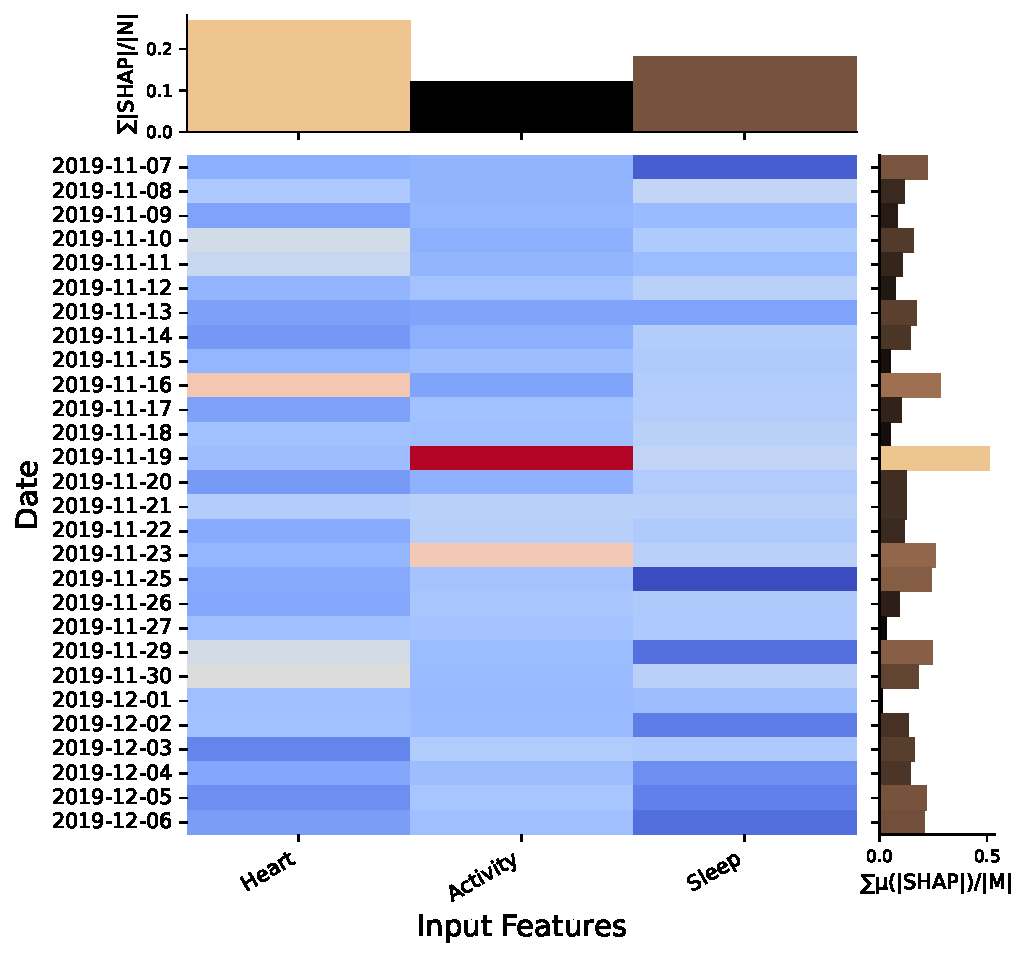
\includegraphics[width=\linewidth]{depression/fig/final_SHAP_comp_SMARTWATCH_combined_ucsd19.pdf}
 \caption{SHAP heatmap for the Smartwatch model}
 \label{fig:part_19_smartwatch}
 \end{subfigure}
 \hfill
 \begin{subfigure}{0.48\linewidth}
 \centering
 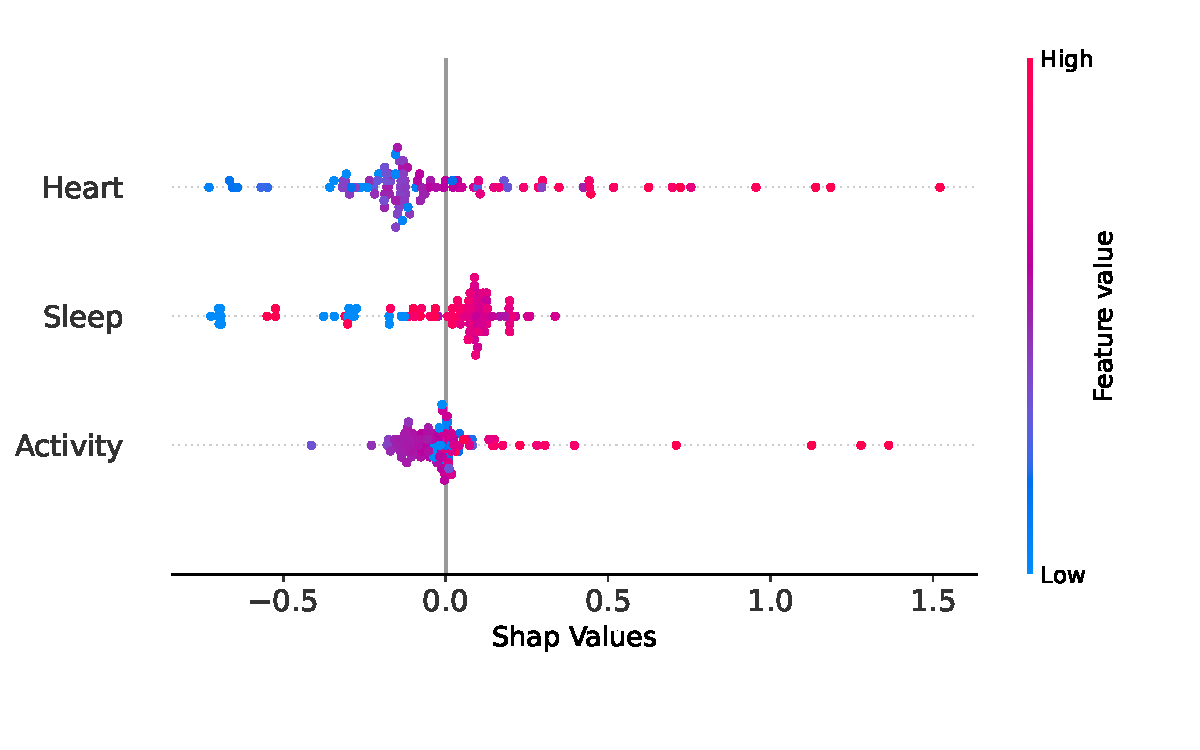
\includegraphics[width=\linewidth]{depression/fig/final_SHAP_summary_comp_SMARTWATCH_combined_ucsd19.pdf}
 \caption{SHAP summary for the Smartwatch model}
 \label{fig:part_19_smartwatch_summary}
 \end{subfigure}

 \vspace{0.5em} % Optional spacing between rows

 % Bottom row: Food figures
 \begin{subfigure}{0.48\linewidth}
 \centering
 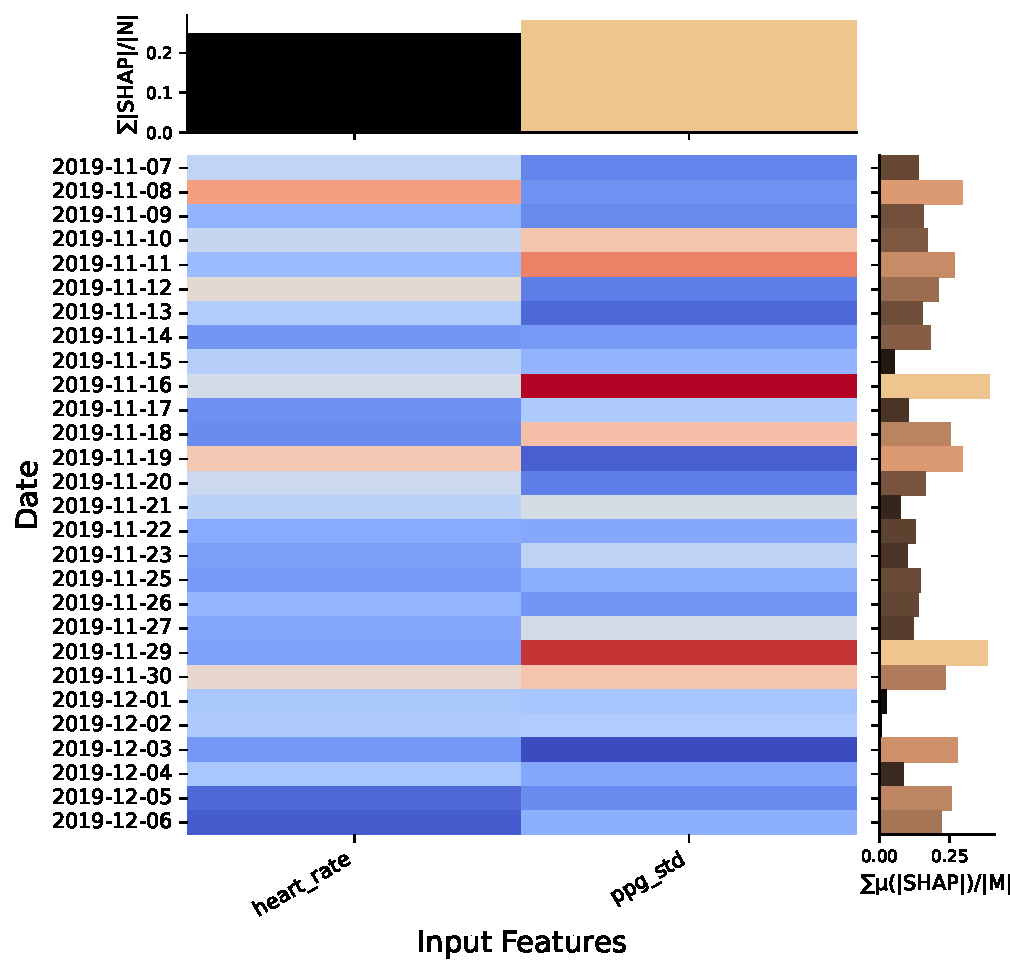
\includegraphics[width=\linewidth]{depression/fig/final_SHAP_comp_heart_combined_ucsd19.pdf}
 \caption{SHAP heatmap for the Heart model}
 \label{fig:part_19_heart}
 \end{subfigure}
 \hfill
 \begin{subfigure}{0.48\linewidth}
 \centering
 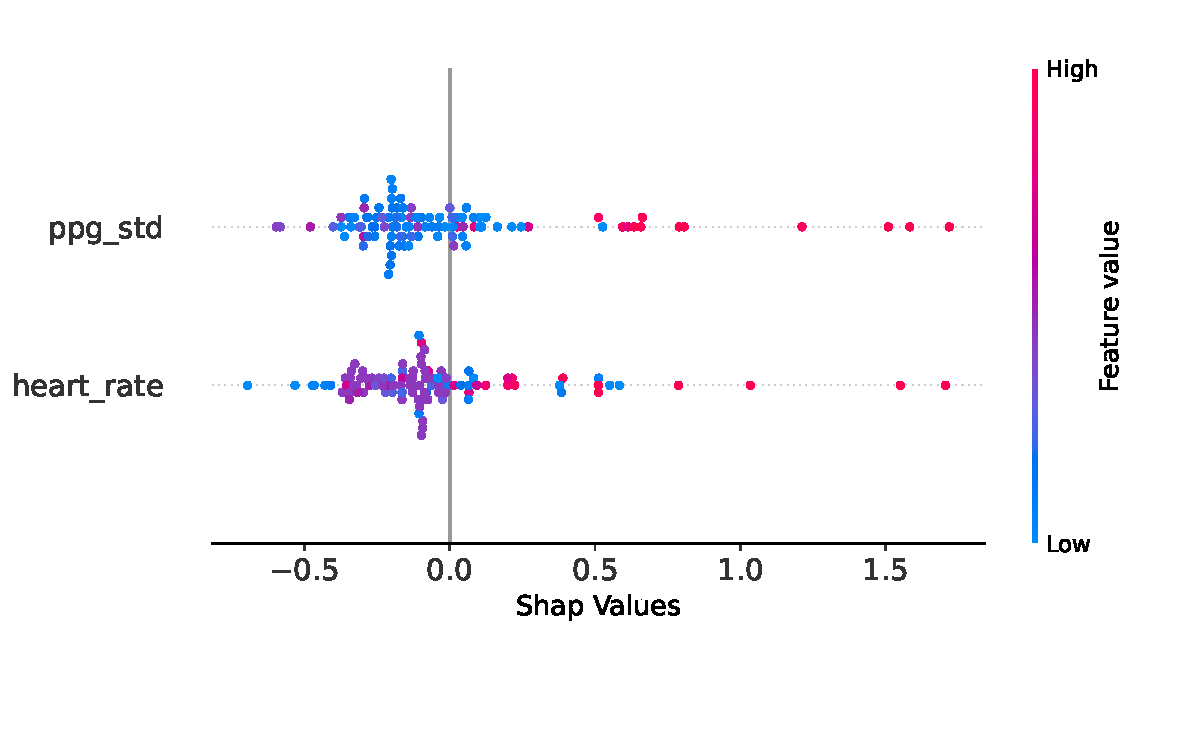
\includegraphics[width=\linewidth]{depression/fig/final_SHAP_summary_comp_heart_combined_ucsd19.pdf}
 \caption{SHAP summary for the Heart model}
 \label{fig:part_19_heart_summary}
 \end{subfigure}

 \caption{SHAP heatmaps and summary plots for Stage2 (top row), Smartwatch (middle row), and Heart (bottom row) clusters for participant UCSD19 and Approach 3.}
 \label{fig:shap_ucsd19_approach3}
\end{figure}




Figure \ref{fig:shap_ucsd19_approach3} is obtained using the top-down approach. First, we compute the top model (from Stage 2) feeding into the Merge model using SHAP values, which is \emph{Smartwatch model}. We then compute the top features for the \emph{Smartwatch model} merge model and find that the \emph{Heart} cluster model is the most influential. Continuing this exercise, we find that \emph{ppg\_std} or heart-rate-variability is the most influential feature. This observation indicates that for Participant 19, the input Smartwatch super-cluster is the most influential, particularly the heart-rate-variability feature from its Heart cluster.

Furthermore, the heatmap over the days shows that the effect of \emph{ppg\_std} on the participant mood score prediction was mostly negative. This indicates that this feature mainly contributes to reducing mood score prediction and is associated with improving the participant's mood. If needed, other cluster models can also be similarly analysed for their best input features. 

Moreover, the SHAP summary plots from figure  \ref{fig:part19_stage2_summary} show that, on the whole, a higher value of the three Stage 2 merge models' outputs increases the value of the mood score prediction (more depressed). Smartwatch is the most influential cluster, followed by EMA and Neurocognitive. Similarly (from figure  \ref{fig:part_19_smartwatch_summary}),  on the whole, a higher value of the three Stage 1 cluster models that feed into the Smartwatch model increases the value of the mood score prediction (more depressed). Heart is the most influential cluster, followed by Sleep and Activity. Finally (From figure(\ref{fig:part_19_heart_summary}), we also find that lower heart-rate-variability and generally lower heart rate are associated with a lower mood score prediction for this participant. These insights can then be used to tailor personalised interventions. \newline



\begin{figure}[htbp]
 \centering

 % Top row: Merge figures
 \begin{subfigure}{\linewidth}
 \centering
 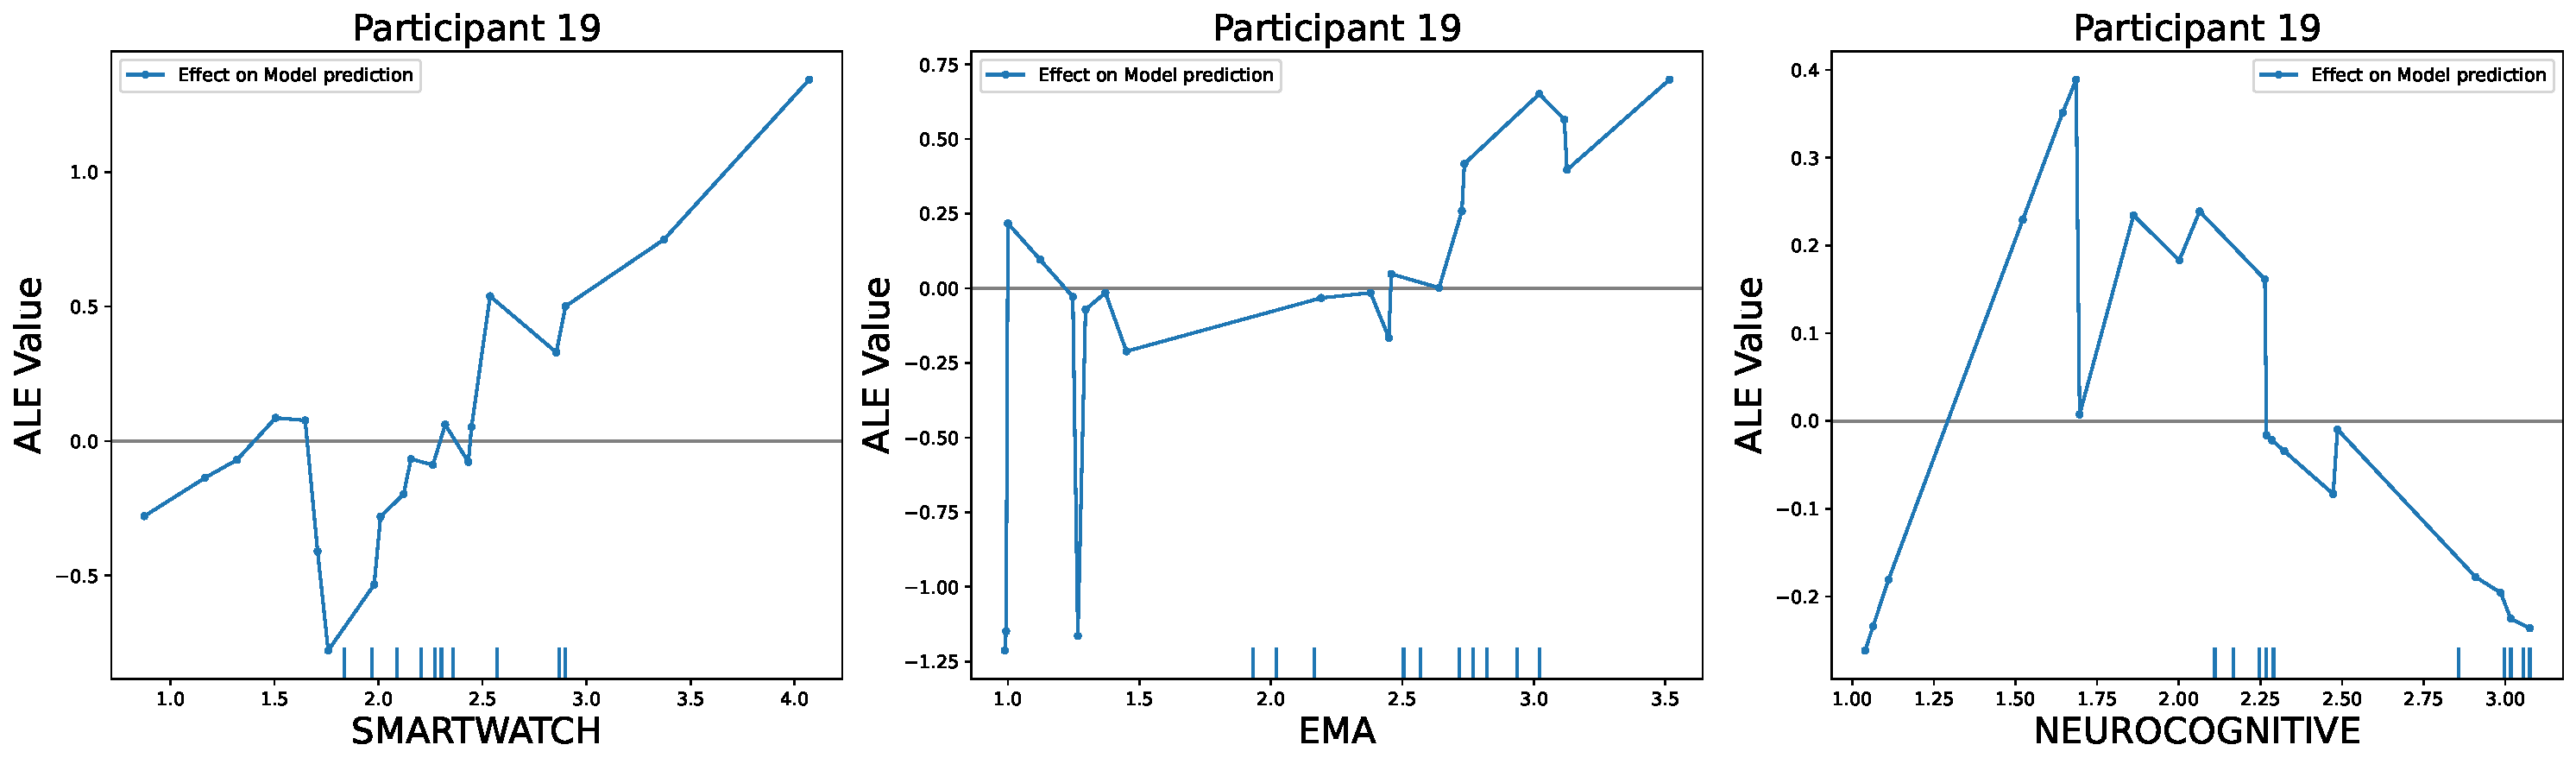
\includegraphics[width=\linewidth]{depression/fig/Final_ALEOverall_comp_ucsd19_Stage2_argmax.pdf}
 \caption{ALE plot for the Merge model}
 \label{fig:part19_stage2_ale}
 \end{subfigure}
 \vspace{0.5em}
 \begin{subfigure}{\linewidth}
 \centering
 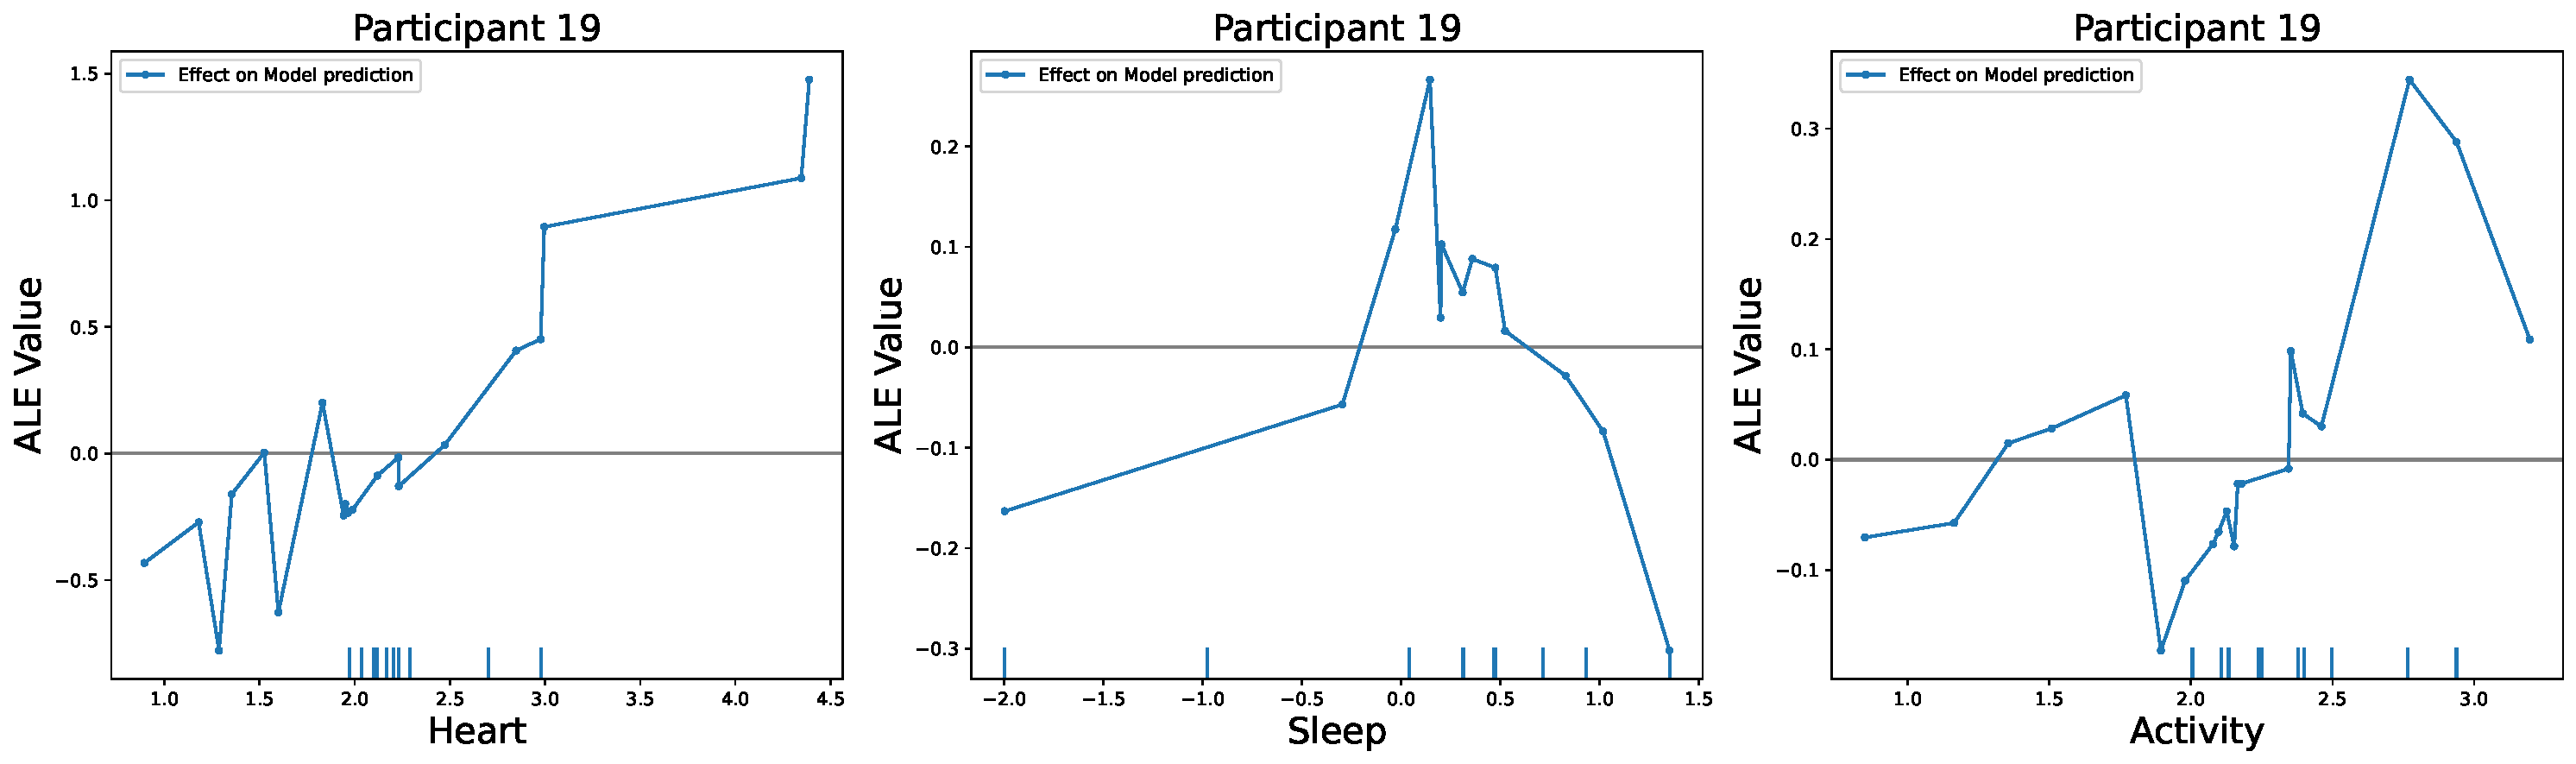
\includegraphics[width=\linewidth]{depression/fig/Final_ALEOverall_comp_ucsd19_SMARTWATCH_argmax.pdf}
 \caption{ALE plot for the Smartwatch model}
 \label{fig:part19_smartwatch_ale}
 \end{subfigure}
 \vspace{0.5em}
 \begin{subfigure}{\linewidth}
 \centering
 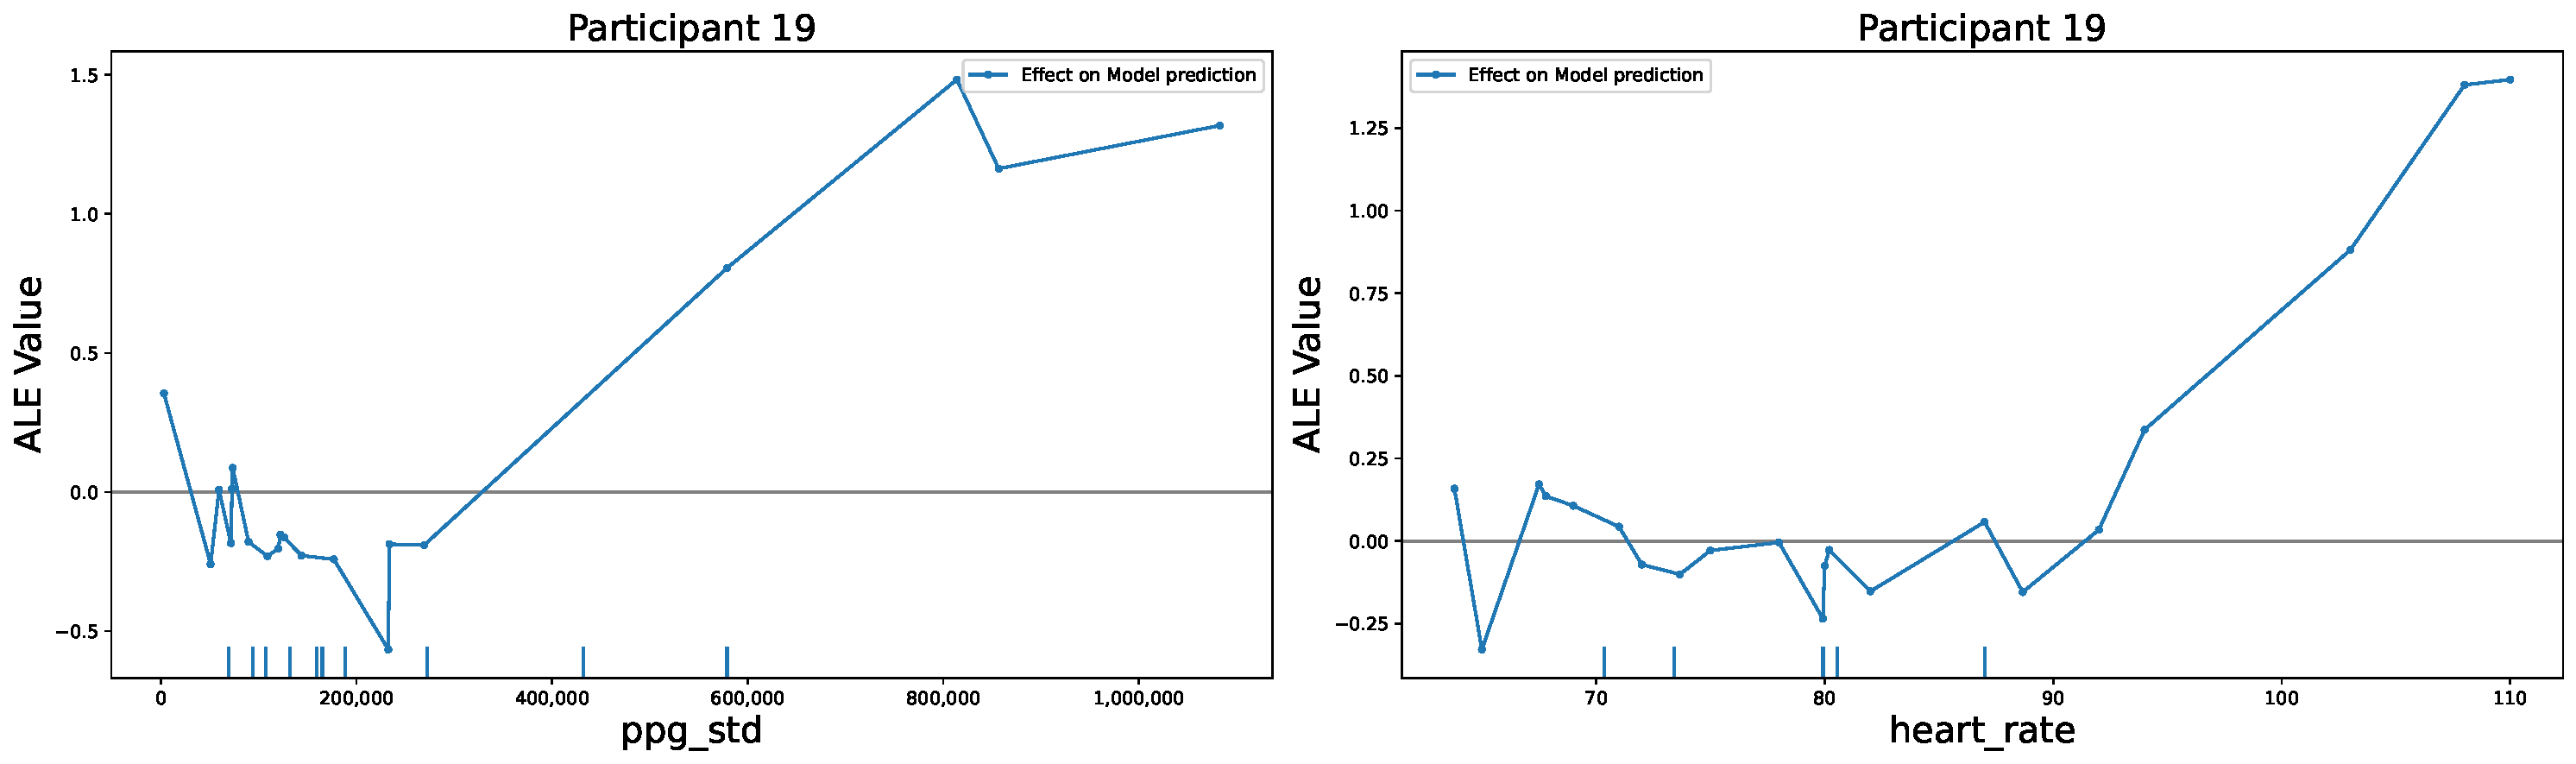
\includegraphics[width=\linewidth]{depression/fig/Final_ALEOverall_comp_ucsd19_heart_argmax.pdf}
 \caption{ALE plot for Heart}
 \label{fig:part19_heart_ale}
 \end{subfigure}
 \caption{ALE plots for Participant 19 and Approach 3}
 \label{fig:ale_ucsd19_approach3}
\end{figure}


\underline{\textit{ALE Plots for top features:}} 

Figure \ref{fig:ale_ucsd19_approach3} shows the ALE plots for the top input features for the Merge and Diet models obtained using the SHAP analysis discussed in the previous section. A positive value (or negative value) in the plot implies an increase (or decrease) in mood-score prediction.

Figure \ref{fig:ale_ucsd19_approach3} shows the ALE plots for the top input features for the Merge, Smartwatch and Heart models obtained using the SHAP analysis discussed in the previous section. We can see from the figure that the Smartwatch and EMA models, which feed into the Merge model, have an overall increasing trend, indicating that a higher value will most likely increase the mood score (which makes depression worse). However, the Neurocognitive model has an increasing trend for lower values and a decreasing trend for higher values, indicating that Neurocognitive input features that ensure that the model outputs a low or high value can help reduce mood scores.

Also, the ALE plots for the Heart and Activity, which feed into the best Stage 2 model (Smartwatch) model, have an increasing trend. However, the Sleep model does not, indicating that more sleep than baseline sleep can help improve mood. Finally, we see that both \emph{ppg\_std} and \emph{heart\_rate} from the Heart model contribute to a lower mood score only if their values are lower. For higher values, they increase the mood score. Thus, it is prudent to make sure that activities that keep the heart rate below 90 and the \emph{ppg\_std} below 300,000 are used to manage the mood of this participant. \newline 





\underline{\textit{Anchors for Explanation:}} 

Lastly, we demonstrate how Anchors can explain changes in mood scores by identifying the most relevant decision rules—based on the underlying features—that apply to each prediction. For example, suppose a participant's mood rating jumps by 2 points (say, from 2 to 4), indicating a sudden worsening of depressive symptoms. In that case, we can explain the prediction at the moment of change and just before it. By examining the IF-THEN rules generated by Anchors for the periods preceding and following the prediction,  we can find which feature alterations likely drove the mood shift. Please note that anchors only explain individual mood predictions, which cannot be generalised over the whole dataset.


\begin{equation}\label{eq:anchor19_3}
\begin{split}
\text{IF }&\;\bigl((\text{Smartwatch} \le 1.90)
    \;\land\; (\text{EMA} \le 2.31)
    \;\land\; (\text{Neurocognitive} > 2.11)\bigr),\\
 &\quad\text{THEN }Depressed = 2,\;\ Precision = 0.96,\;\ Coverage = 0.01;\\[6pt]
\text{IF }&\;\bigl((1.90 < \text{Smartwatch} \le 2.80)
    \;\land\; (\text{EMA} \le 2.58)\bigr),\\
 &\quad\text{THEN }Depressed = 3,\;\ Precision = 0.96,\;\ Coverage = 0.45.
\end{split}
\end{equation}




\begin{equation}\label{eq:anchor19_4}
\begin{split}
\text{IF }&\;\bigl((\text{Sleep} \le -0.30)
    \;\land\; (\text{Heart} \le 1.98)
    \;\land\; (\text{Activity} \le 2.20)\bigr),\\
 &\quad\text{THEN }Depressed = 2,\;\ Precision = 0.94,\;\ Coverage = 0.03;\\[6pt]
\text{IF }&\;\bigl((\text{Activity} > 2.05)
    \;\land\; (1.98 < \text{Heart} \le 2.83)
    \;\land\; (\text{Sleep} \le 0.83)\bigr),\\
 &\quad\text{THEN }Depressed = 3,\;\ Precision = 0.96,\;\ Coverage = 0.44.
\end{split}
\end{equation}

\begin{equation}\label{eq:anchor19_5}
\begin{split}
\text{IF }&\;\bigl((117501.12 < \text{ppg\_std} \le 270472.29)
    \;\land\; (74.97 < \text{heart\_rate} \le 80.00)\bigr),\\
 &\quad\text{THEN }Depressed = 2,\;\ Precision = 0.50,\;\ Coverage = 0.17;\\[6pt]
\text{IF }&\;\bigl((\text{ppg\_std} \le 140671.59)
    \;\land\; (\text{heart\_rate} \le 92.00)\bigr),\\
 &\quad\text{THEN }Depressed = 3,\;\ Precision = 0.99,\;\ Coverage = 0.55.
\end{split}
\end{equation}



Let us consider the case/data point where the mood score for Participant 19 increases from two to three in 4 hrs. We first find the anchor rules for the Merge model, followed by those for the Smartwatch model (the best model of the Merge model). Finally, we compute the anchor rules for the best model for the Smartwatch model, which is the Heart cluster model. We can also find the anchor rules for other cluster models (if needed), but we avoid them here for conciseness. 

In equations \ref{eq:anchor19_3}, \ref{eq:anchor19_4}, and \ref{eq:anchor19_5}, we present the anchor rules for the Merge model, Smartwatch model and the Heart model, respectively, where the first set of conditions pertains to the case when the mood score is 2, and the second set is when the score is 3. If we compare the anchor rules, we can see that, in this instance, a higher mood score/depressive mood is associated with a higher value of the Smartwatch model output, a higher value of the Heart and Activity models, and a lower value of feature \emph{ppg\_std} and a slightly higher heart rate. Thus, ensuring a lower heart rate variability and heart rate through lower activity and monitoring using a smartwatch shows potential in managing the mood of this participant. These rules can be monitored over a few days to extract patterns in the rules and decide on the best intervention.


\subsubsection{Clinical Significance and Comparison with Monolithic Models}

Overall, the compositional model explainability approach allows a clinician to focus on the most important feature groups and features of a model in a guided hierarchical manner. For instance, in the case of Participant 19, if the clinician wants to obtain the most influential features for the compositional model, they can focus on the SMARTWATCH model, followed by the Heart model and finally the \emph{ppg\_std} and \emph{heart\_rate} features due to the separation of features and the sub-models used to form the compositional model. This analysis reveals that reducing the heart rate variability and heart rate, both monitored using a smartwatch, shows potential in managing the mood of this participant. A clinician can then use anchor rules to extract the exact range of these features associated with a lower mood score. 

Similarly, a clinician may focus on other models, such as the EMA model, followed by its best input models and features. As presented in the previous sections, additional hierarchical analyses of mood changes can be performed to obtain more insights. In fact, the very design of compositional models allows a clinician to choose a cluster model instead of the whole compositional model if the cluster model is found expressive enough or if a smaller model is needed.

Such analyses are impossible with a monolithic model, where the clinician must focus on the large monolithic model and all its input features, as there is no separation of features and the MLP neurons used to form the model. All neurons are interconnected, and this makes individual analysis of features difficult. Even though SHAP and other approaches can be used to analyse the monolithic model, they may fail to disentangle the feature importances when features are multicollinear. 

This limitation with monolithic models could explain the differences in the top features between the monolithic (Diet) and compositional (Heart) models for Participant 19. However, the effect of differences in model architecture and the explainability techniques (which are model dependent) used to analyse the models could also explain the differences in the top features. Overall, monolithic models require that the clinician have a deeper understanding of the model and the explainability techniques to obtain a correct analysis and interpretation of the model behaviour. 


\subsection{Discussion}
\label{sec:depression_results_discussion}

The monolithic and compositional results show that personalised mood score prediction benefits from MLP models over the baseline classifiers reported in Section~\ref{sec:depression_results}, and that decomposition can improve both error metrics and interpretability for a subset of participants. Table~\ref{tab:performance_comparison} shows compositional MLPs matching or beating monolithic \gls{mae} for several participants (e.g.\ P-10, P-14, P-18, P-20, P-23, P-24, P-26), while monolithic models remain stronger for others (e.g.\ P-1, P-15). There was no single compositional approach (1, 2, or 3) that was uniformly best across the cohort; hyperparameter optimisation was applied per model, but the experiments did not search automatically over the number of stages or cluster groupings, so the reported architectures are illustrative rather than globally optimal.

The explainability results help explain why compositional designs were pursued alongside raw accuracy. For Participant~19, hierarchical SHAP, ALE, and Anchor analyses route attention through the merge model to the smartwatch branch and then to heart-related features, rather than spreading importance across all inputs in one monolithic MLP. That pattern is difficult to obtain when every feature competes within a single network, even with post-hoc methods, and it matches the clinical reading in Section~\ref{sec:depression_compositional_results}: lower heart-rate variability and activity may associate with higher mood scores for this individual. Monolithic explanations for the same participant emphasise diet-related inputs instead, which is consistent with entangled features in one model rather than with compositional structure alone being wrong.

Compositionality also changes how explanations should be used in practice. Cluster-level sub-models allow SHAP, ALE, and Anchors to be applied within sleep, activity, or heart domains, supporting focused intervention advice and easier identification of which branch underperforms. Merge models remain less transparent than leaf clusters; clusters may not capture cross-domain interactions unless the merge stage learns them, and training several models increases computational cost. Results depend on imputation, missing wearable readings, and short longitudinal records per participant; explainability here describes associations learned by the model, not established causes, and should be checked across SHAP, ALE, and Anchors when predictive performance is modest.

Relative to the autonomous driving case study in Chapter~\ref{chapter:av}, this application does not close a real-time control loop over a physical plant. It still fits the broader \gls{cps} setting described in Chapter~\ref{chapter:background}: wearable and phone sensors measure behavioural and physiological state, software processes those signals, and outputs (mood scores and explanations) inform monitoring and self-management. Processing is offline on stored trajectories, which precludes the same \gls{wcet} and enforcement guarantees as the \gls{av} chapter, but it reflects how many health analytics systems are deployed. In this context, compositional modelling mainly advances personalised prediction and explainability rather than hard real-time safety bounds.


\section{Summary}\label{sec:depression_conclusions}

In this chapter, we introduced monolithic and compositional modelling and explainability frameworks for personalised mood score prediction from multimodal data. Using a one-month dataset of 14 mild to moderately depressed participants, we imputed missing values, trained and optimised MLP models with eight evolutionary and statistical algorithms, validated performance with 5-fold cross-validation, and compared SHAP, ALE, and Anchors explanations at personal and population levels.

Compositional MLPs improved or matched monolithic performance for many participants while providing hierarchical, cluster-aligned explanations that monolithic models do not support directly. The framework is model-agnostic and can be extended to other architectures and modalities. Future work includes explainability for temporal dynamics, automated selection of compositional architectures, and evaluation on larger longitudinal cohorts.









